%!TEX TS-program = pdflatexmk
%% V1.4b
%% 2015/08/26
%% by Michael Shell
%% See:
%% http://www.michaelshell.org/
%% for current contact information.
%%
%%
%% Support sites:
%% http://www.michaelshell.org/tex/ieeetran/
%% http://www.ctan.org/pkg/ieeetran
%% and
%% http://www.ieee.org/

%%*************************************************************************
%% Legal Notice:
%% This code is offered as-is without any warranty either expressed or
%% implied; without even the implied warranty of MERCHANTABILITY or
%% FITNESS FOR A PARTICULAR PURPOSE! 
%% User assumes all risk.
%% In no event shall the IEEE or any contributor to this code be liable for
%% any damages or losses, including, but not limited to, incidental,
%% consequential, or any other damages, resulting from the use or misuse
%% of any information contained here.
%%
%% All comments are the opinions of their respective authors and are not
%% necessarily endorsed by the IEEE.
%%
%% This work is distributed under the LaTeX Project Public License (LPPL)
%% ( http://www.latex-project.org/ ) version 1.3, and may be freely used,
%% distributed and modified. A copy of the LPPL, version 1.3, is included
%% in the base LaTeX documentation of all distributions of LaTeX released
%% 2003/12/01 or later.
%% Retain all contribution notices and credits.
%% ** Modified files should be clearly indicated as such, including  **
%% ** renaming them and changing author support contact information. **
%%*************************************************************************





\documentclass[10pt,journal,compsoc]{IEEEtran}

%
% manually specify the path to it like:
% \documentclass[10pt,journal,compsoc]{../sty/IEEEtran}




% Some very useful LaTeX packages include:
% (uncomment the ones you want to load)


% *** MISC UTILITY PACKAGES ***
%
%\usepackage{ifpdf}
% compilation based on whether the output is pdf or dvi.
% usage:
% \ifpdf
%   % pdf code
% \else
%   % dvi code
% \fi
% http://www.ctan.org/pkg/ifpdf
% \ifCLASSINFOpdf conditional that works the same way.
% have to be run twice to clear warning/error messages.


% !TEX root =  paper.tex

% \usepackage{cite}
% \usepackage{amsmath,amssymb,amsfonts}
% \usepackage{algorithmic}
% \usepackage{graphicx}
% \usepackage{subcaption}
% \usepackage{textcomp}
% \usepackage{xcolor}
% \usepackage{multicol} % \columnbreak
% \usepackage{balance}
% \usepackage{enumitem}    
%\usepackage[table]{xcolor}
%\usepackage{nohyperref}

\usepackage{xcolor}

\usepackage{tabularx} 
\usepackage{collcell}

% \usepackage[usenames,dvipsnames,svgnames,table,xcdraw]{xcolor}
% \usepackage[usenames,dvipsnames,svgnames]{xcolor}
% \usepackage{pgfplots}
% \pgfplotsset{compat=1.10}


\usepackage{booktabs}
\usepackage[caption=false,font=normalsize,labelfont=sf,textfont=sf]{subfig}
%\usepackage{cite}
% \usepackage{hyperref}
\usepackage{array}
\usepackage{threeparttable}
\usepackage{enumitem}    
\usepackage[greek,english]{babel}
\usepackage{ifthen}
\usepackage{xspace}
\usepackage{fancybox}
\usepackage{marginnote}
\usepackage{tcolorbox}
\usepackage{multirow}
\usepackage{mathtools}
\usepackage{algpseudocode, algorithm, algorithmicx}
\usepackage{color}
\usepackage{soul}
\usepackage{graphicx}
\usepackage{amsmath}
\usepackage{tikz}
\usepackage{cleveref}
\usepackage{hhline}
\usepackage{balance}

\usepackage{listings}
\usepackage{parcolumns}
\usepackage{cleveref}

\usepackage{array}

\usepackage{adjustbox}
\usepackage{flushend}
\usepackage[switch]{lineno}
\definecolor{light-gray}{gray}{0.95}
\newcommand{\code}[1]{\colorbox{light-gray}{\fontsize{9pt}{10pt}\texttt{#1}}}

\definecolor{circled-color}{gray}{0.15}
\newcommand*\circled[1]{\tikz[inner sep=.1ex,baseline=-.75ex] \node[circle,draw,color=white,fill=circled-color] {#1};}


\def\BibTeX{{\rm B\kern-.05em{\sc i\kern-.025em b}\kern-.08em
    T\kern-.1667em\lower.7ex\hbox{E}\kern-.125emX}}
\newboolean{showcomments}
\setboolean{showcomments}{true}
\hypersetup{draft,bookmarks=false}

\ifthenelse{\boolean{showcomments}}
{
	\definecolor{myyellow}{RGB}{255, 228, 26}
	\definecolor{myblue}{RGB}{50, 50, 220}
	\newcommand{\nb}[2]{
		{\sf
			\fcolorbox{myyellow}{yellow}{\scriptsize\textbf{#1}}%
			$\blacktriangleright$%
			{\color{myblue}\fontsize{7pt}{8pt}\selectfont\textbf{#2}}%
		}%
	}
}
{
	\newcommand{\nb}[2]{}
}


\newcommand{\Mo}[1]{\nb{Mo}{#1}}
\newcommand{\Ali}[1]{\nb{Ali}{#1}}


\usepackage{color}


\definecolor{editorGray}{rgb}{0.95, 0.95, 0.95}
\definecolor{editorOcher}{rgb}{1, 0.5, 0} % #FF7F00 -> rgb(239, 169, 0)
\definecolor{editorGreen}{rgb}{0, 0.5, 0} % #007C00 -> rgb(0, 124, 0)

\lstdefinelanguage{JavaScript}{
  morekeywords={typeof, new, true, false, catch, function, return, null, catch, switch, var, if, in, while, do, else, case, break},
  morecomment=[s]{/*}{*/},
  morecomment=[l]//,
  morestring=[b]",
  morestring=[b]'
}
\lstdefinelanguage{HTML5}{
        language=html,
        sensitive=true, 
        alsoletter={<>=-},
        otherkeywords={
        % HTML tags
        <html>, <head>, <form>, </form>, <div>, </div>, <p>, </p>, 
        <span>, </span>, <input, <textarea, </textarea>, <select, </select>, 
        <option>, </option>, <title>, </title>, <meta, />, </head>, <body>,
        <canvas, \/canvas>, <script>, </script>, </body>, </html>, <!, html>, <section>, </section>
        },  
        ndkeywords={
        % General
        =,
        % HTML attributes
        charset=, id=, width=, height=, type=, value=, checked
        % CSS properties
        border:, transform:, -moz-transform:, transition-duration:, transition-property:, transition-timing-function:
        },  
        morecomment=[s]{<!--}{-->},
        tag=[s]
}

\lstdefinelanguage{CSS}{
  morekeywords={background,color,display,justify,content,font,weight,border,size,padding},
  morestring=[s]{:}{;},
  sensitive,
  morecomment=[s]{/*}{*/}
}
\newcommand{\todo}[1]{\textcolor{magenta}{\nb{TODO:}{#1}}}
\newcommand{\header}[1]{\par\smallskip\noindent\textbf{#1.}}
\newcommand{\toolname}{\textsc{AxeForm}\xspace}
\newcommand{\html}{\textsc{HTML}\xspace}
\newcommand{\css}{\textsc{CSS}\xspace}
\newcommand{\javascript}{\textsc{JavaScript}\xspace}
\lstset{%
    % Basic design
    backgroundcolor=\color{editorGray},
    basicstyle={\linespread{1.0}\scriptsize\ttfamily},   
    frame=l,
    % Line numbers
    xleftmargin={0.75cm},
    numbers=left,
    stepnumber=1,
    firstnumber=1,
    numberfirstline=true,
    % Code design   
    keywordstyle=\color{blue}\bfseries,
    commentstyle=\color{darkgray}\ttfamily,
    ndkeywordstyle=\color{editorGreen}\bfseries,
    stringstyle=\color{editorOcher},
    % Code
    language=HTML5,
    alsolanguage=JavaScript,
    alsodigit={.:;},
    tabsize=2,
    showtabs=false,
    showspaces=false,
    showstringspaces=false,
    extendedchars=true,
    breaklines=true,        
    % Support for German umlauts
    literate=%
    {Ö}{{\"O}}1
    {Ä}{{\"A}}1
    {Ü}{{\"U}}1
    {ß}{{\ss}}1
    {ü}{{\"u}}1
    {ä}{{\"a}}1
    {ö}{{\"o}}1
}






%\usepackage{showframe}

% *** CITATION PACKAGES ***
%
\ifCLASSOPTIONcompsoc
  % requires cite.sty v4.0 or later (November 2003)
  %\usepackage[nocompress]{cite}
\else
  % normal IEEE
  %\usepackage{cite}  
\fi
% \cite{} output to follow that of the IEEE. Loading the cite package will
% result in citation numbers being automatically sorted and properly
% "compressed/ranged". e.g., [1], [9], [2], [7], [5], [6] without using
% cite.sty will become [1], [2], [5]--[7], [9] using cite.sty. cite.sty's
% \cite will automatically add leading space, if needed. Use cite.sty's
% such as if a citation ever needs to be enclosed in parenthesis.
% cite.sty is already installed on most LaTeX systems. Be sure and use
% The latest version can be obtained at:
% http://www.ctan.org/pkg/cite
% The documentation is contained in the cite.sty file itself.
%
% Note that some packages require special options to format as the Computer
% Society requires. In particular, Computer Society  papers do not use
% compressed citation ranges as is done in typical IEEE papers
% (e.g., [1]-[4]). Instead, they list every citation separately in order
% (e.g., [1], [2], [3], [4]). To get the latter we need to load the cite





% *** GRAPHICS RELATED PACKAGES ***
%
\ifCLASSINFOpdf
  % \usepackage[pdftex]{graphicx}
  % declare the path(s) where your graphic files are
  % \graphicspath{{../pdf/}{../jpeg/}}
  % and their extensions so you won't have to specify these with
  % every instance of \includegraphics
  % \DeclareGraphicsExtensions{.pdf,.jpeg,.png}
\else
  % will default to the driver specified in the system graphics.cfg if no
  % driver is specified.
  % \usepackage[dvips]{graphicx}
  % declare the path(s) where your graphic files are
  % \graphicspath{{../eps/}}
  % and their extensions so you won't have to specify these with
  % every instance of \includegraphics
  % \DeclareGraphicsExtensions{.eps}
\fi
% installed on most LaTeX systems. The latest version and documentation
% can be obtained at: 
% http://www.ctan.org/pkg/graphicx
% Another good source of documentation is "Using Imported Graphics in
% http://www.ctan.org/pkg/epslatex
%
%
% You can find documentation about the pdfTeX application at:
% http://www.tug.org/applications/pdftex






% *** MATH PACKAGES ***
%
%\usepackage{amsmath}
% A popular package from the American Mathematical Society that provides
% many useful and powerful commands for dealing with mathematics.
%
% thus preventing page breaks from occurring within multiline equations. Use:
%\interdisplaylinepenalty=2500
% version and documentation can be obtained at:
% http://www.ctan.org/pkg/amsmath





% *** SPECIALIZED LIST PACKAGES ***
%
%\usepackage{algorithmic}
% This package provides an algorithmic environment fo describing algorithms.
% You can use the algorithmic environment in-text or within a figure
% environment to provide for a floating algorithm. Do NOT use the algorithm
% floating environment provided by algorithm.sty (by the same authors) or
% algorithm float types and packages that provide these will not provide
% correct IEEE style captions. The latest version and documentation of
% algorithmic.sty can be obtained at:
% http://www.ctan.org/pkg/algorithms
% Also of interest may be the (relatively newer and more customizable)
% http://www.ctan.org/pkg/algorithmicx




% *** ALIGNMENT PACKAGES ***
%
%\usepackage{array}
% the standard LaTeX2e array and tabular environments to provide better
% appearance and additional user controls. As the default LaTeX2e table
% generation code is lacking to the point of almost being broken with
% respect to the quality of the end results, all users are strongly
% advised to use an enhanced (at the very least that provided by array.sty)
% set of table tools. array.sty is already installed on most systems. The
% latest version and documentation can be obtained at:
% http://www.ctan.org/pkg/array


% generate multiline equations as well as matrices, tables, etc., of high
% quality.




% *** SUBFIGURE PACKAGES ***
%\ifCLASSOPTIONcompsoc
%  \usepackage[caption=false,font=footnotesize,labelfont=sf,textfont=sf]{subfig}
%\else
%  \usepackage[caption=false,font=footnotesize]{subfig}
%\fi
% for subfigure.sty, the latter of which is no longer maintained and is
% in non-IEEE style figure/table captions. To prevent this problem, be sure
% handling of captions.
% Note that the Computer Society format requires a sans serif font rather
% than the serif font used in traditional IEEE formatting and thus the need
%
% http://www.ctan.org/pkg/subfig




% *** FLOAT PACKAGES ***
%
%\usepackage{fixltx2e}
% in the LaTeX2e kernel, the most notable of which is that in current
% LaTeX2e releases, the ordering of single and double column floats is not
% single column figure to be placed prior to an earlier double column
% figure.
% needed.
% The latest version and documentation can be found at:
% http://www.ctan.org/pkg/fixltx2e


%\usepackage{stfloats}
% the ability to do double column floats at the bottom of the page as well
% as the top. (e.g., "\begin{figure*}[!b]" is not normally possible in
% LaTeX2e). It also provides a command:
%\fnbelowfloat
% to enable the placement of footnotes below bottom floats (the standard
% LaTeX2e kernel puts them above bottom floats). This is an invasive package
% which rewrites many portions of the LaTeX2e float routines. It may not work
% with other packages that modify the LaTeX2e float routines. The latest
% version and documentation can be obtained at:
% http://www.ctan.org/pkg/stfloats
% \baselineskip to stretch. Authors submitting work to the IEEE should note
%
% \usepackage{dblfloatfix}
% The latest version can be found at:
% http://www.ctan.org/pkg/dblfloatfix




%\ifCLASSOPTIONcaptionsoff
%  \usepackage[nomarkers]{endfloat}
% \let\MYoriglatexcaption\caption
% \renewcommand{\caption}[2][\relax]{\MYoriglatexcaption[#2]{#2}}
%\fi
% endfloat.sty was written by James Darrell McCauley, Jeff Goldberg and 
% figures/tables without any captions are placed on a page by themselves at
% the user used the short optional argument of \caption[]{}.
% \let\MYorigsubfloat\subfloat
% \renewcommand{\subfloat}[2][\relax]{\MYorigsubfloat[]{#2}}
% avoid the use of subfigure captions (many IEEE journals avoid them anyway)
% and instead reference/explain all the subfigures within the main caption.
% The latest version of endfloat.sty and its documentation can obtained at:
% page by themselves.




% *** PDF, URL AND HYPERLINK PACKAGES ***
%
%\usepackage{url}
% systems. The latest version and documentation can be obtained at:
% http://www.ctan.org/pkg/url
% Basically, \url{my_url_here}.





% *** Do not adjust lengths that control margins, column widths, etc. ***
% (Unless specifically asked to do so by the journal or conference you plan
% to submit to, of course. )


% correct bad hyphenation here
%\hyphenation{op-tical net-works semi-conduc-tor}


\begin{document}

%
% paper title
% Titles are generally capitalized except for words such as a, an, and, as,
% at, but, by, for, in, nor, of, on, or, the, to and up, which are usually
% not capitalized unless they are the first or last word of the title.
% Do not put math or special symbols in the title.
%\title{Computer Vision in Software Engineering: \\ A Systematic Literature Review}
%\title{Computer Vision in Software Engineering: \\ A Survey}
\title{\changed{A Survey on the Use of Computer Vision to Improve Software Engineering Tasks}}
%
%
% author names and IEEE memberships
% note positions of commas and nonbreaking spaces ( ~ ) LaTeX will not break
% a structure at a ~ so this keeps an author's name from being broken across
% two lines.
% use \thanks{} to gain access to the first footnote area
% a separate \thanks must be used for each paragraph as LaTeX2e's \thanks
% was not built to handle multiple paragraphs
%
%
%\IEEEcompsocitemizethanks is a special \thanks that produces the bulleted
% lists the Computer Society journals use for "first footnote" author
% affiliations. Use \IEEEcompsocthanksitem which works much like \item
% \IEEEcompsocitemizethanks becomes like \thanks and
% facilitates dual compilation, although admittedly the differences in the
% desired content of \author between the different types of papers makes a
% journal papers have the author affiliations above the "Manuscript

\author{Mohammad~Bajammal,
        Andrea~Stocco,~\IEEEmembership{Member,~IEEE Computer Society}, % <-this % stops a space
        Davood~Mazinanian
        and~Ali~Mesbah,~\IEEEmembership{Member,~IEEE Computer Society}% <-this % stops a space
\IEEEcompsocitemizethanks{%
\IEEEcompsocthanksitem Mohammad Bajammal, Davood Mazinanian, and Ali Mesbah are with the University of British Columbia, Vancouver, BC, Canada. \protect\\
% note need leading \protect in front of \\ to get a newline within \thanks as
% \\ is fragile and will error, could use \hfil\break instead.
\IEEEcompsocthanksitem Andrea Stocco is with the Universit\`{a} della Svizzera Italiana, Switzerland.}% <-this % stops an unwanted space

%\thanks{Manuscript received April 19, 2005; revised August 26, 2015.}
}
%\email{{bajammal,astocco,dmazinanian,amesbah}@ece.ubc.ca}

% note the % following the last \IEEEmembership and also \thanks - 
% these prevent an unwanted space from occurring between the last author name
% and the end of the author line. i.e., if you had this:
% 
%                     ^------------^------------^----Do not want these spaces!
%
% a space would be appended to the last name and could cause every name on that
% line to be shifted left slightly. This is one of those "LaTeX things". For
% instance, "\textbf{A} \textbf{B}" will typeset as "A B" not "AB". To get
% "AB" then you have to do: "\textbf{A}\textbf{B}"
% \thanks is no different in this regard, so shield the last } of each \thanks
% that ends a line with a % and do not let a space in before the next \thanks.
% Spaces after \IEEEmembership other than the last one are OK (and needed) as
% you are supposed to have spaces between the names. For what it is worth,
% this is a minor point as most people would not even notice if the said evil
% space somehow managed to creep in.



% The paper headers
\markboth{IEEE TRANSACTIONS ON SOFTWARE ENGINEERING,~Vol.~XY, No.~X, XYZ~2020}%
{Bajammal \MakeLowercase{\textit{et al.}}: Computer Vision in Software Engineering: A Systematic Literature Review}
% The only time the second header will appear is for the odd numbered pages
% 
% *** Note that you probably will NOT want to include the author's ***
% *** name in the headers of peer review papers.                   ***
% You can use \ifCLASSOPTIONpeerreview for conditional compilation here if
% you desire.



% The publisher's ID mark at the bottom of the page is less important with
% Computer Society journal papers as those publications place the marks
% outside of the main text columns and, therefore, unlike regular IEEE
% journals, the available text space is not reduced by their presence.
% If you want to put a publisher's ID mark on the page you can do it like
% this:
%\IEEEpubid{0000--0000/00\$00.00~\copyright~2015 IEEE}
% or like this to get the Computer Society new two part style.
%\IEEEpubid{\makebox[\columnwidth]{\hfill 0000--0000/00/\$00.00~\copyright~2015 IEEE}%
%\hspace{\columnsep}\makebox[\columnwidth]{Published by the IEEE Computer Society\hfill}}
% Remember, if you use this you must call \IEEEpubidadjcol in the second
% papers don't need this extra clearance.)



% use for special paper notices
%\IEEEspecialpapernotice{(Invited Paper)}



\begin{abstract}

Filling web forms is a common online activity. 
Web forms are made accessible to users with disabilities 
by conveying their content through specific DOM labeling 
markups. The absence of these markups is one of the most 
common accessibility errors. However, there is currently 
little to no work in terms of having an automated analysis 
process that allows inferring the labeling markups in order 
to automatically make forms accessible for users with disabilities. 
In this paper, we propose a web form analysis approach that 
infers labels by first constructing different types of 
visual cues from a form, then optimizing the combination of 
various cues and form fields, and finally augmenting the DOM 
to incorporate the required labeling markup. We evaluate 
our approach on real-world subjects and assess the accuracy 
of labeling inference, the safety of the DOM augmentation, 
as well as the labeling performance. The results show an 
average F1-measure of 88.4\% for label inference, and an 
average run-time of around 1.6 seconds.

\end{abstract}

\keywords{web forms, accessibility errors, 
accessibility repair, visual analysis}



% make the title area
\maketitle


% To allow for easy dual compilation without having to reenter the
% abstract/keywords data, the \IEEEtitleabstractindextext text will
% - because all conference papers position the abstract like regular
% papers do.
\IEEEdisplaynontitleabstractindextext
% \IEEEdisplaynontitleabstractindextext has no effect when using



% For peer review papers, you can put extra information on the cover
% page as needed:
% \ifCLASSOPTIONpeerreview
% \begin{center} \bfseries EDICS Category: 3-BBND \end{center}
% \fi
%
% creates the second title. It will be ignored for other modes.
\IEEEpeerreviewmaketitle



% !TEX root =  paper.tex

\section{Introduction}
\label{section:introduction}

The development of user interfaces (UIs) for web apps is often a manual and time 
consuming task.In a survey of more than 5,700 developers, 51\% reported working 
on app UI design tasks on a daily basis~\cite{IDC:survey},
more so than other development tasks, which they tended to perform every few days. 
Another study also showed that an average of 48\% of the code size of software is 
related to the user interface~\cite{myers:ui:survey}.

A common workflow for creating web user interfaces 
is \textit{mockup based design}~\cite{Newman:2000:SitemapsStoryboardsSpecifications, Ozenc:2010:SupportDesigners}.
In this approach, a graphic designer creates a rough illustration of the anticipated UI design, called the \textit{mockup} or \textit{wireframe},
usually through a graphic design software or a WYSIWYG editor. 
This mockup is then exported to \html to be rendered in a browser.
A web developer then examines the mockup and begins constructing web components for the app, which are nowadays implemented in one of the popular front-end frameworks such as \angular~\cite{Angular} or \react~\cite{React}.

\renewcommand{\toolname}{\textsc{VizMod}\xspace}
The main building block of UI design, and a cornerstone of these front-end frameworks, is the concept of  
\textit{reusable components}~\cite{React-components, Angular-components},
which are a set of APIs and coding practices allowing reuse and encapsulation of repeated patterns on the front-end.
Reusable components help improve modularity and maintainability, make the code more testable, and effectively remove duplication,
by offloading the task of creating repetitive patterns to the web browser at runtime. 
Recent surveys show that using front-end frameworks is extensively popular among web developers. In one survey more than 92\% of around 28,000 surveyed web developers stated that they use a framework 
rather than constructing UIs using pure \html~\cite{StateOfJS:WebPlatformTests}.
As a result, creating reusable components is often an essential element of building an app's front-end.

This component creation process can often be time consuming and tedious~\cite{thinking:in:components} in practice;  
 it requires several manual steps,
including the examination of the mockup, 
checking potential elements that may or may not be suitable for conversion to components, 
constructing a template for components that unifies repeated segments, 
adding placeholders for variable content, and
refactoring the code to replace instances with instantiated components~\cite{thinking:in:components}.

To the best of our knowledge, there has been little to no automated support in creating these reusable web components from mockups. Existing techniques help to manage mockups themselves, but do not generate any components. For instance, one set of approaches~\cite{Sinha:2013:CompilingMockupsToFlexibleUIs, ramon2016layout} takes a mockup as input
and converts its layout into a responsive code (e.g., through CSS) such that it is flexible  to maintain the layout on different
display sizes. Others~\cite{mihalcea2014const_with_mockups} propose a tool that overlays the mockup as a transparency layer while implementing the UI, 
and performs a snapping-like functionality that aligns against various parts of the mockup.

In this chapter, we propose a technique, implemented in a tool, \toolname, to fill this gap by automatically generating reusable web components from mockups.
Given a web mockup, our technique automatically identifies patterns on the UI,  refactors the \html code, and creates reusable components for popular front-end frameworks that are already familiar to developers such as \react or \angular. At the core of our approach is an unsupervised machine learning process for the detection of reusable UI patterns; we use features composed of a hybrid of information obtained from the Document Object Model (DOM) 
as well as the visual analysis of the UI.

We evaluate \toolname on \numberOfTemplates real-world web mockups by automatically identifying and transforming \totalNumberOfComponentInstances component instances 
into \numberOfComponents components.    
We also ask \numberOfParticipants experts to manually
find patterns on the mockups
and compare the output from our approach with the manually-identified patterns.
Our approach is able to achieve \precision precision and \recall recall, on average, in correctly detecting reusable patterns in the UIs. 


This chapter makes the following main contributions:
\begin{itemize}
	\item A novel approach for automatically generating web components (e.g., \react, \angular) from mockups, which is the first to address this issue, to the best of our knowledge.
	\item An implementation of our approach, available in a tool called \toolname.
	\item A qualitative and quantitative evaluation of \toolname in terms of its accuracy and reusability of the generated components. 
	
\end{itemize}


 



% !TEX root =  manuscript.tex
\section{Prior Work}\label{sec:related}

To the best of our knowledge, 
there are no existing surveys or systematic literature reviews that 
share a similar goal to this chapter. 
\hl{
This section discusses  
a broader range of research areas in order to put 
the survey in its proper context.
We therefore begin by discussing secondary studies concerning 
computer vision-based techniques 
in various non-software engineering fields. 
While such studies are not directly related to our topic of discussion, 
they help place the survey within wider context of other similar surveys. 
Second, we explore other surveys that 
are interdisciplinary in nature, 
given the interdisciplinary nature of our survey.
Finally, we discuss visual GUI testing 
techniques, an area with a relatively large 
number of papers employing visual analysis techniques. 
}


\header{Surveys on Computer Vision-based Engineering}
In this subsection, we discuss some of the surveys or systematic literature reviews 
concerning the use of computer vision in various engineering fields. 
We note that these are non-software engineering fields 
(e.g., aerospace or automotive engineering) 
and are included here for the sake of completeness. 

Kumar~\cite{cv-fabric-defect} catalogues the 
fabric defect detection methodologies reported 
in about 150 references into three main categories: 
statistical, spectral and model-based. 
They conclude that despite the significant progress 
in last decade, the problem of fabric defect detection 
still remains challenging and requires effort by 
combining existing approaches. 
%
Kanellakis and Nikolakopoulos~\cite{cv-for-uavs} 
present a comprehensive literature review on vision 
based applications for unmanned aerial vehicles (UAVs) focusing mainly on current 
developments and trends. Computer vision techniques are used 
mainly for visual localization and mapping, 
obstacle detection and avoidance, aerial target 
tracking, and guidance. Among the limitations, 
it is mentioned that the algorithms are based on 
rigid assumptions such as low speed vehicles 
that do not account for fast scene alterations. 
Thus, the main challenge is to design solutions 
that can quickly react to ever changing sceneries, 
characterized by a high degree of dynamism and evolution. 
%
Liu and Dai~\cite{5508131} discuss solutions 
for UAVs from three main families, namely visual 
navigation, aerial surveillance and airborne 
visual simulation.
%
Al-Kaff et al.~\cite{ALKAFF2018447} provide another 
survey of techniques for UAVs, particularly 
visual navigation algorithms, obstacle detection 
and avoidance and aerial decision-making. It is 
mentioned that artificial perception applications 
have represented important advances in the latest 
years in the expert system field related to unmanned aerial vehicles. 

Gandhi and Triveli~\cite{1706871} discuss the recent 
research on pedestrian detection and collision 
prediction. Among the information gathered by 
the various sensors, the camera's image is one 
of the most used, along with visual analysis 
techniques for behaviour modelling in accident 
prediction, direction estimation, and collision prediction. 
%
Brunetti et al.~\cite{BRUNETTI201817} discuss 
vision-based pedestrian detection systems pertaining 
to three different application fields: video 
surveillance, human-machine interaction and 
analysis. Notably, they discuss both the 
differences between 2D and 3D vision systems, 
and indoor and outdoor systems.
%
Janai et al.~\cite{DBLP:journals/corr/JanaiGBG17} 
provides a comprehensive survey on problems, 
datasets, and methods in computer vision for 
autonomous vehicles. First, they overview the 
datasets and benchmarks used in autonomous 
driving research. Then, the discuss the state 
of the art on several relevant topics, 
including recognition, reconstruction, motion 
estimation, tracking, scene understanding, and 
end-to-end learning.

\header{Interdisciplinary Surveys in SE}
Interdisciplinary surveys are often used to collect 
and analyze a body of knowledge across the boundaries 
between two or more fields. 
Here, we discuss some of the 
surveys or systematic literature reviews that have analyzed scientific and social 
fields from a software engineering perspective. 

Zhang et al.~\cite{Zhang-TSE} provide a comprehensive 
survey of techniques for testing machine learning systems. 
The survey covers 144 papers on different 
testing properties such correctness, robustness, 
and fairness, testing components 
(e.g., data, learning program, and frameworks), 
testing workflow (e.g., test generation and 
test evaluation), and application scenarios 
(e.g., autonomous driving, machine translation). 
The paper also analyses trends concerning datasets, 
research trends, and research focus, 
concluding with research challenges and promising 
research directions in machine learning testing.
%
Besz\'{e}des~\cite{Beszdes2019InterdisciplinarySO} 
performed a systematic analysis of fault localization 
literature across different engineering fields, 
with the aim to find solutions in non-software areas 
that could be successfully adapted to software fault 
localization. Among their findings, they indicate that 
some classes of methods in computer networks literature are good 
candidates for adaptation, and could potentially be 
reused for software fault localization. 
%
Van der Linden and Hadar~\cite{8283537} performed a 
systematic literature review of physics of notation applications, 
a conceptual modelling language used for  
requirement specification. They analyzed what 
notations have been evaluated and designed using 
the physics of notation, for what reasons, 
to what degree applications consider requirements 
of their notation's users, and how verifiable these 
applications are. 
%
% Mao et al.~\cite{MAO201757} provide a comprehensive 
% survey of the use of crowdsourcing in software engineering, 
% summarising industrial crowdsourcing practice in software 
% engineering and the corresponding case studies. They 
% further analyzed the software engineering domains, 
% tasks and applications for crowdsourcing and the 
% platforms and stakeholders involved in realizing 
% crowdsourced SE solutions. 

% Similarly to the mentioned works, our survey is also 
% ``approach-oriented'' as it focuses on exploring how 
% approaches from one field (i.e., CV) have been employed 
% in a different field (i.e., SE), for what problems they 
% have been used, and what are the main pros and cons. 
% In contrast, to the best of our knowledge, our treatment 
% of computer vision in software engineering solutions is 
% novel in the software engineering literature, because 
% it comprehensively look at the solutions applied to 
% any stage of the software life cycle. 

Sabaren et al.~\cite{Sabaren-2018-JCST} conduct a systematic 
literature review of cross-browser regression testing.
In their survey, their goal was to collect the 
various techniques that 
have been proposed to perform cross-browser testing. 
The authors also describe several 
challenges in this specific context, such as the 
automatic identification of dynamic components in a 
user interface, which undermines the effectiveness of 
proposed testing techniques, causing many false 
positives in practice.
We note that the survey of~\citet{Sabaren-2018-JCST} has  
found 11 papers that happened to be in our final pool of \numberOfPapers 
collected papers. This is a happenstance since our survey 
has a different objective for the following reasons. 
The work by~\citet{Sabaren-2018-JCST} answers the following
question: what approaches have been used to 
conduct cross-browser regression testing.
In contrast, our work is not concerned at all with that problem. 
Our work answers the following question: in what ways have computer 
vision been used to advance software engineering. 
The reason we had some common papers is because regression testing 
happened to be an area where visual techniques were found 
to be particularly useful. 
However, in terms of the scope and objective, there is no overlap.
%
In other words, \citet{Sabaren-2018-JCST} focus on a specific 
problem (i.e., cross-browser regression testing), regardless 
of what approaches were used (e.g., DOM analysis, 
state space navigation, visual analysis). 
That is, the survey in \citet{Sabaren-2018-JCST} is 
\emph{problem-specific} but approach-agnostic. 
In contrast, our survey is \emph{approach-specific} but 
problem-agnostic. Any overlap between the two surveys is because 
some papers happen to be in the pool of both surveys, 
but not because both surveys perform the same objective or have 
the same research questions. 
We focus on a specific approach 
(i.e., computer vision techniques), but consider its 
potential for any area of software engineering 
(e.g., testing, maintenance, development, design, requirements). 
In summary, none of the aforementioned surveys have a similar 
goal as that of this chapter. 

\header{Visualization Research}
Visualization is the process of creating diagrams, charts, or any other 
kind of representation, from a given dataset. 
Visualization is part of any scientific process regardless of the field, 
and therefore has also been used in software engineering. 
There are a number of surveys on the use of visualization
in various aspects of software engineering,
such as surveys on visualization for software security~\cite{wagner2015survey,zhang2012survey},
surveys on visualization for static analysis~\cite{caserta2010visualization},
development coordination~\cite{storey2005use},
maintenance and evolution~\cite{novais2013software, koschke2003software},
to name a few. 
Visualization, however, is not the scope of this survey. 

\header{Visual GUI Testing}
Issa et al~\cite{6320526} first introduced the notion of
\textit{visual testing} as a subset of traditional GUI testing.
In their analysis, the authors conducted a study of bugs
in four open source systems, and found that visual bugs
represent between 16\% and 33\% of reported defects in those systems. 
In recent years, researchers and practitioners have started
conducting empirical experiments aiming at understanding the
comparative performance of a few visual testing approaches. 
For instance, Al\'{e}groth et al.~\cite{alegroth2017,
alegroth2015conceptualization}
present a case study of the benefits and challenges of
using visual GUI testing by the team at one software company. 
In another study, Al\'{e}groth et al.~\cite{8367046} study 
the applicability and feasibility of Visual GUI testing in 
an industrial Continuous Integration environment, describing the 
main challenges faced by researchers to make it effective in practice. 
Garousi et al.~\cite{garousi2017comparing} compare two popular visual
testing tools (Sikuli and JAutomate) in one industrial project,
and go through differences in test creation process, execution,
and maintenance.

All such works analyze different technical and social aspects 
related to the use of Visual GUI testing in a specific context 
(i.e., the development and maintenance of test code). 
In contrast, our work is agnostic to any specific area or context. 
That is, it does not aim to focus on GUI testing. 
Rather, the goal is to broadly examine the use of visual techniques 
across any software engineering area (e.g., requirements, design, 
development, testing, maintenance) and for any task (e.g., refactoring, 
reverse engineering, regression testing). 


\begin{figure*}
    \centering
    %\fbox{
    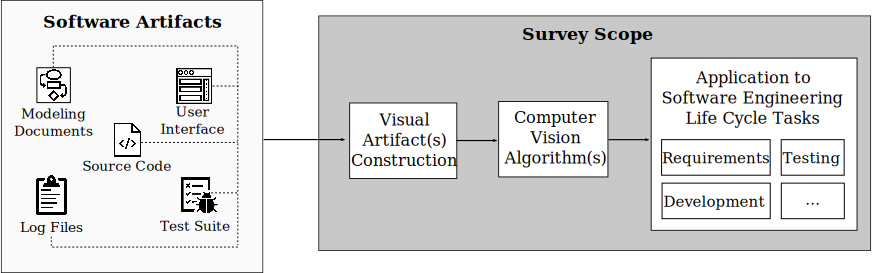
\includegraphics[scale=0.50]{survey/figures/scope-horizontal}
    %}
    \caption{Overview of the scope of this survey.}
    \label{fig:scope}
\end{figure*}





% !TEX root =  manuscript.tex
\section{Methodology}\label{sec:methodology}

In order to conduct the survey in a thorough
and structured manner, we follow the established
guidelines by Kitchenham et al.~\cite{kitchenham2007guidelines}.
We begin by introducing terminology
and concepts needed to understand the remainder
of this survey.
Next, we define the scope of the work
and flesh it out into specific research questions
we aim to answer in this survey.
We then describe the details of the paper
collection process. 
Finally, we specify the inclusion and exclusion criteria
applied to select the most relevant body of work 
from the existing literature. 

\subsection{Definitions}\label{sec:defs}

In order to categorize
the use of visual approaches in software engineering, 
we use the terms \textit{areas} and \textit{tasks}.
Software engineering areas are the various stages in the software
lifecycle~\cite{IEEEComputerSociety:2014:GSE:2616205}.
Examples of SE areas include software requirements, software design,
and software testing.
Within each area, different \textit{tasks} can be defined.
Each task is a specific activity that aims to
achieve a well-defined objective related to that area.
For instance, we refer to unit testing or regression testing as
SE tasks within the software testing SE area,
whereas code migration or code refactoring are tasks within
software maintenance area.
Accordingly, the rationale for using these two terms is
to discuss our findings in more precise levels of granularity,
in order to be able to analyze the findings across areas and
for tasks within a specific area.

Next, we define the following terms in order to clarify
which aspect of computer vision is being discussed:

\begin{defn}[\textbf{Visual Artifact}]
\textit{A visual artifact is any datum %of information 
that satisfies the following two conditions: 
(1)~it constitutes a digital image or video, and
(2)~it is associated with one or more software engineering area(s).}
\end{defn}

\begin{defn}[\textbf{Visual Approach}]
\textit{A visual approach is an algorithm designed to solve a software engineering problem,
which takes as input one or more visual artifacts, 
then typically incorporates a computer vision method or similar techniques as one or more of its steps,
and finally yields an output that is used to achieve a software engineering task.
}
\end{defn}

The rationale for defining these two terms is to have
precision and clarity when describing how visual analysis is used to 
solve a software engineering problem.
We use the term \emph{visual approach} to indicate 
that the approach used to solve an SE problem 
is based on analyzing visual data pertaining to the software.
We use the term \emph{visual artifact} to refer to software artifacts
that are visual in nature, to differentiate them from other
software artifacts that are non-visual (e.g., log files,
requirements documents). 
The link between the two terms is that 
visual artifacts are the visual data consumed
by a visual approach.
Similarly, a visual approach is the algorithm
that needs visual artifacts as input. 
To clarify all of the aforementioned terms,
we give a simple example.  
Consider the case of cross-browser testing,
where the goal is to check whether a given
web app is being rendered identically in different browsers.
Visual approaches for cross-browser testing
often take a screenshot of the app in a set of 
different browsers, and then visually compare the screenshots.
In this case,
screenshots are the visual artifacts used or extracted
from the software,
and screenshot image comparison is the visual approach used to 
solve the SE task of cross-browser testing.

\subsection{Scope}\label{sec:scope}

The scope of this work is to conduct a survey
to help structure, curate, and unify
the dispersed literature in this research area,
and to analyze how computer vision techniques have
been used in software engineering,
and what challenges were reported when they were used. 
This would help shed light on the potential of these 
techniques, and make them more visible and accessible.

\changed{
\autoref{fig:scope} illustrates the scope of this work
in relation to the software engineering life cycle
and other software artifacts. 
The figure should be viewed as a multi-step process, 
beginning with visual artifacts construction, and ending with 
an application to a software engineering task, 
as defined in Section~\ref{sec:defs}.  
As shown in the figure,
the scope is to survey the following aspects: 
(1)~how are visual artifacts (defined in Section~\ref{sec:defs})
constructed or acquired from the software?  
%
This aspect is included in the scope because constructing or acquiring 
visual artifacts is the first step in a computer vision 
processing pipeline, and therefore should be explored 
in order to have a well-rounded survey.
%
(2)~what computer vision algorithms are used to analyze or 
process the constructed visual artifacts? 
% 
This aspect is included in the scope because examining the visual 
processing or analysis conducted in order to address a given paper's 
research questions yields insight into how visual techniques 
can be potentially applied to various tasks of software engineering.
%
(3)~what are the software engineering areas and tasks
where visual approaches have been used?

The figure also helps clarify what areas are outside the scope
of this survey.
For instance, the scope is not concerned with works where 
computer vision techniques were not utilized, 
or works that do not use any visual artifacts. 
Section \ref{sec:inclusions} fleshes out the scope into a detailed set of 
inclusion and exclusion criteria. 
}


\subsection{Research Questions}
As discussed in Section \ref{sec:scope},
the scope is to survey the use of computer vision
in solving software engineering problems.
In this section, we flesh out the scope
into the following specific research questions:

RQ1: What are the main software engineering areas and tasks
for which computer vision approaches have been used to date? 
We formulate this RQ in order to build a high level
picture of the areas of software engineering where computer vision
approaches were used. This aims at identifying potential trends
of areas with high adoption of computer vision 
and conversely areas where little to no computer vision approaches were used.
This can help the software engineering community in identifying
potential gaps in the utilization of computer vision for software engineering. 

RQ2: Why are computer vision approaches adopted? 
We formulate this RQ in order to identify common rationales 
for using computer vision to solve software engineering problems.
This understanding of why computer vision approaches
were used can subsequently help identify new software engineering
areas or tasks where similar problems and rationales exist
and therefore potentially benefiting from computer vision approaches.

RQ3: How are computer vision approaches applied to software and its visual artifacts? 
This RQ is a natural progression of the previous RQs. 
The previous RQs identified the rationales of using computer vision 
and the SE areas where computer vision were used.
This RQ examines the ``how.''
That is, the mechanism(s) by which computer vision was applied to software.
This can help guide the implementation of computer vision approaches
to solve software engineering problems.

RQ4: How are software engineering tasks that leverage computer vision techniques evaluated? 
This RQ examines the methods used to evaluate the use of computer vision approaches
in software engineering problems, as well as a summary of the reported limitations and challenges.
This may help with selecting an evaluation strategy when exploring the use of a computer vision approach,
and informing adopters of potential challenges.

\begin{figure*}
    \centering
    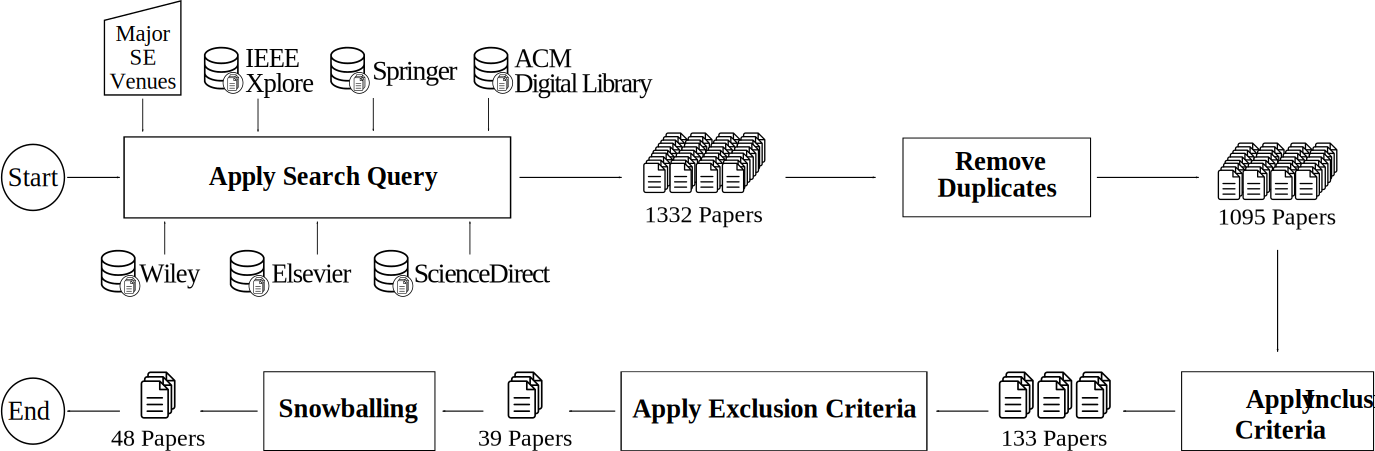
\includegraphics[width=0.80\textwidth]{survey/figures/overview}
    \caption{Overview of the paper collection process. }
    \label{fig:overview}
\end{figure*}

\subsection{Paper Collection}\label{sec:collection}

\autoref{fig:overview} shows our paper search and selection process.
In order to collect as much relevant literature as possible, 
we used two types of sources for paper collection: 
paper repository databases, and major software engineering venues.

\header{Paper Repository Databases}
To conduct our search, we used the databases of the following
well-known publishers of scientific literature:
IEEE Xplore, ACM Digital Library, ScienceDirect, Springer, Wiley, and Elsevier.
The search covers papers that have been published until June 2020. 
We used more than one database to ensure collecting
as many papers as possible from all known publishers.

\header{Software Engineering Venues}
The preceding selection of paper repositories
aims at casting a wide net in order to capture as many
relevant literature as possible.
However, since the databases contain an extremely large
number of papers, it is possible that papers 
relevant to our survey are lost in the vast number of returned papers.

For this reason, and in order to make sure we collect highly relevant papers, we complemented the database search with a manual issue-by-issue search within the conference proceedings and journal articles from 
top-tier software engineering venues (listed in \autoref{tbl:paper-sources}).
The final pool of collected papers is the combined list of papers from both the database search and the SE venues search.

\changed{
\header{Interdisciplinary Venues}
Given the interdisciplinary nature of this work, 
we also performed manual issue-by-issue search within 
the conference proceedings of relevant fields, namely, 
computer-human interaction, computer vision and machine 
learning. We selected the top three venues (based on the h5 index from Google Scholar) from each field.
The searched venues are listed in the last section of
 \autoref{tbl:paper-sources} (under ``Interdisciplinary Venues'').
}

\header{Search Query} For each of the aforementioned sources, 
we performed a search query using various combinations
of terms to retrieve papers in different software engineering areas
that are potentially using computer vision.
The query was performed on all data fields of the paper,
returning matches to either the \emph{title}, \emph{abstract},
\emph{keywords}, or \emph{text} of the paper.
The query is composed of two parts: keywords related to the approach
and keywords of the various software engineering areas.
Keywords of the approach include strings such as
``computer vision'' or ``visual''.
They were included in the query in order to indicate
our interest in works that use computer vision or visual approach.
Keywords describing the areas include strings such as
``development'' or ``testing'' or any of the software engineering
life cycle phases (e.g., requirements, maintenance).
The final applied search query is as follows:
%\begin{quote}
\emph{{[}computer vision {OR} image processing 
{OR} image analysis {OR} visual{]}
\ \ {AND}\ \ 
{[}requirements {OR} design {OR} development 
{OR} testing {OR} maintenance {OR} comprehension {]}}
%\end{quote}
The result of this query led to an initial pool of \initialPoolSize papers,
which was further filtered in the next stages.

\header{Duplicates removal}
During the paper collection step, we aimed to be
thorough by including as many paper sources as possible
in order to capture all potentially relevant works.
However, this resulted in many duplicate papers since a given
paper might be included in more than one database and venue.
Therefore, we filtered the collected pool
of papers by removing duplicate works based on their titles.

\subsubsection{Inclusion and Exclusion Criteria}\label{sec:inclusions} 
The search conducted on the databases and venues is, 
by design, very inclusive. This allows us to collect as many
papers as possible in our pool. 
However, this generous inclusivity results in having papers that are not directly
related to the scope of this survey.
Accordingly, we define a set of specific inclusion and exclusion criteria
and apply them to each paper in the pool, and remove papers not meeting the criteria.
This ensures that each collected paper is inline with our scope and research questions.

\header{Inclusion criteria}
We define the following inclusion criteria: 
%
(1)~The paper should be contributing to any stage
of the software engineering process,
whether in early requirements and modeling,
through development and design, or finally testing and maintenance.
We included this criteria in order to focus on software engineering papers.
This is because we found a notable number of computer vision papers 
that were in fields other than software engineering (e.g., biology).
%
(2)~The paper should include a computer vision processing of the software or its artifacts.
That is, the work achieves its objective (whether partially or fully) by extracting,
analyzing, or processing visual artifacts pertaining or relevant to the software.
This is an important and key criterion for paper selection because it ensures
we meet the core scope of our survey. 
%
(3)~The paper should be a full technical research paper that has a
detailed description of the visual approach utilized.
This criterion is imposed in order to have sufficient information to answer our research questions.
Answering our research questions, such as RQ3 and RQ4, requires that 
we examine technical software engineering research papers,
as opposed to, for instance,
technical magazine articles, industrial white papers, or similar grey literature
which do not have sufficient level of detail.
Some demo/short papers can be allowed if they have dedicated and detailed 
sections discussing the detailed mechanism of the visual approach and its
evaluation. 
This enables creating a pool of papers that have
rich and detailed information and findings,
in order to answer key research questions related to
the details of the visual approach, the process of creating visual artifacts,
and evaluation strategies. 
%
(4)~The paper should contain a section dedicated to illustrating
some form of quantitative or qualitative evaluation of the technique,
or an illustration of its use case. 
This criterion was imposed in order to enable us to
fully answer and explore our research questions regarding evaluation strategies.

These criteria were applied 
in a group review process by the authors.
For each paper in the pool, each author initially checked the title and abstract,
and briefly examined the proposed approach and results to ensure that it meets the inclusion criteria.
If this check was not sufficient to conclusively decide
whether the paper should be included in the pool,
we proceeded with a secondary in-depth examination of
the paper's objective, methodology, and evaluation to ensure that the inclusion criteria were met.
Finally, a discussion among the authors was triggered,
to decide on the inclusion of the paper in the final list of works.
 
% !TEX root =  manuscript.tex

\begin{table}

\revised{0.99\textwidth}{

\caption{Conference proceedings and journals considered for paper collection (in addition to database search).}
\centering
% \small % bigger
\scriptsize %smaller
% \tiny % much smaller
\renewcommand{\arraystretch}{1.2}
\setlength{\tabcolsep}{2.5pt}

\begin{tabular}{l l p{7.5cm}}
	\toprule
	& \textbf{Acronym}   & \textbf{Venue}                                                                                              \\ \midrule
	\multirow{18}{*}{\rotatebox{90}{\textbf{SE Conferences}}}
	& ICSE          & International Conference on Software Engineering                                                            \\
	& FSE           & International Symposium on Foundations of Software Engineering                                  \\
	& ESEC/FSE	    & Joint European Software Engineering Conference and Symposium on the Foundations of Software Engineering \\
	& ASE           & International Conference on Automated Software Engineering                                         \\
	& ESEM          & International Symposium on Empirical Software Engineering and Measurement                         \\
	& ICST          & International Conference on Software Testing, Verification and Validation                              \\
	& ISSTA         & International Symposium on Software Testing and Analysis                                        \\
	& MSR           & International Conference on Mining Software Repositories                                                    \\
	& RE            & International Requirements Engineering Conference                                                      \\
	& ICSME         & International Conference on Software Maintenance and Evolution                                          \\
	& MODELS        & International Conference on Model Driven Engineering Languages and Systems                         \\
	& ISSRE         & International Symposium on Software Reliability Engineering                                            \\
	& EASE          & Evaluation and Assessment in Software Engineering                                                           \\
	% & UIST          & ACM Symposium on User Interface Software and Technology                                                     \\
	% & WWW           & International World Wide Web conference                                                                     \\
	% & WSDM          & ACM International Conference on Web Search and Data Mining                                                  \\
	% & ICWE          & International Conference on Web Engineering                                                                 \\
	% & CHI           & ACM CHI Conference on Human Factors in Computing Systems                                                    \\ \midrule
	\midrule
	\multirow{12}{*}{\rotatebox{90}{\textbf{SE Journals}}}
	& TSE           & Transactions on Software Engineering                                                                   \\
	& EMSE          & Empirical Software Engineering                                                                              \\
	& TOSEM         & Transactions on Software Engineering and Methodology                                                    \\
	& JSS           & Journal of Systems and Software                                                                             \\
	% & JVLC          & Journal of Visual Languages and Computing                                                                   \\
	& JSEP          & Journal of Software: Evolution and Process                                                                  \\
	& STVR          & Software Testing, Verification and Reliability                                                              \\
	& ASE           & Automated Software Engineering                                                                              \\
	& IEEE SOFTWARE & IEEE Software                                                                                               \\
	& IET SOFTW.    & IET Software                                                                                                \\
	& IST           & Information and Software Technology                                                                         \\
	& SQJ           & Software Quality Journal                                                                                    \\ 


	\midrule
	
	\multirow{10}{*}{\rotatebox{90}{\textbf{Interdisciplinary Venues}}}
	& CHI       & Conference on Human Factors in Computing Systems  	\\
	& CSCW 		& Conference on Computer-Supported Cooperative Work 	\\
	& UbiComp	& Conference on Pervasive and Ubiquitous Computing 		\\ 
	& UIST      & Symposium on User Interface Software and Technology  	\\

	& NeurIPS   & Conference on Neural Information Processing Systems   \\
	& ICLR		& International Conference on Learning Representations  \\
	& ICML		& International Conference on Machine Learning			\\

	& CVPR    & Conference on Computer Vision and Pattern Recognition   \\
	& ECCV	  & European Conference on Computer Vision					\\
	& ICCV		& International Conference on Computer Vision		\\
	
	\bottomrule

	\end{tabular}
	\label{tbl:paper-sources}
}
\end{table}


\header{Exclusion criteria}\label{sec:exclusions}
During our initial experimental test rounds of paper searching,
we observed that a relatively large number of retrieved papers
were on visualization research.
This is understandable and expected because our queries
include terms such as image, visual, and design.

Accordingly, we exclude papers published in the area of software
visualization for the following reasons.
First, the visualization class of algorithms does not
constitute a \emph{visual approach}, as defined in Section~\ref{sec:defs}.
Visualizations do not use any visual artifact of the software \emph{as an input}.
Rather, such work performs a final visual output or visual
representation of a complete, non-visual, approach.
Accordingly, this area of research is excluded
since it would be outside the scope of this work.
We recall that the scope is to survey visual approaches which,
by definition, \emph{consume} visual artifacts pertaining to the software during the
course of running their algorithm or processing.
Second, in addition to visualization being outside the scope of this survey,
it is already a well-known and common aspect of software engineering, 
and plenty of surveys already exist on the use of visualization
in various aspects of software engineering, 
as mentioned in \Cref{sec:related}.

We also exclude commercial software services or open-source tools
that have no corresponding publication, for the following reasons.
First, including services or tools that are not peer-reviewed
would negatively impact our ability to conduct the survey because tools and services 
that are not backed by a publication do not include
a detailed explanation of their approach.
This reduces our ability to answer key research questions for this survey,
such as what specific computer vision techniques were used,
what is the visual artifacts construction process, and 
how were the computer vision algorithms applied to the visual artifacts.
Services and tools without a corresponding publication
also typically do not have a thorough systematic evaluation,
and therefore we are unable to answer research questions related to
how computer vision techniques were evaluated,
what are the main findings, and what were the challenges.


\header{Snowballing}
At the end of searching database repositories and
conference proceedings and journals,
and applying inclusion and exclusion criteria,
we obtained a total of 57 unique papers.
Next, 
to mitigate the risk of omitting relevant literature from this survey,
we also performed backward snowballing~\cite{Wohlin:2014:GSS:2601248.2601268}
by inspecting the references cited by the collected papers so far.
Nine additional papers were retrieved during this phase,
which led to a final pool of 66 unique papers.
\autoref{table:selected-primary-studies}
shows the final pool of papers
that will be discussed and analyzed in the remainder of this work.

% !TEX root =  manuscript.tex

\begin{table}[t]
\caption{Collected data items (Synthesis Matrix)}
\centering
\renewcommand{\arraystretch}{1.2}
\setlength{\tabcolsep}{9pt}
\begin{tabular}{l l}
	\toprule
	\textbf{Field}                    & \textbf{Use}     \\ \midrule
	Title                             & Documentation    \\
	Author(s)                         & Documentation    \\
	DOI identification number         & Documentation   \\
	Abstract                          & Paper Selection \\
	Text                          & Paper Selection \\
	Venue                             & RQ1             \\
	Year                              & RQ1             \\
	% Total number of Citations         & \davood{?}      \\
	Target platform                   & RQ1             \\
	Software engineering area         & RQ1             \\
	Software engineering task         & RQ1             \\
	Reasons for adopting CV approach  & RQ2             \\
	Visual artifact(s) used           & RQ3             \\
	CV algorithm(s) used    	      & RQ3             \\
	Evaluation process \& challenges  & RQ4             \\
	Main results                      & RQ4             \\
	Limitations of CV methods used    & RQ4             \\ \bottomrule
\end{tabular}
	\label{tbl:collected-info}
\end{table}


\header{Extracted Information}
For each retrieved paper,
we collect a set of data necessary to answer the research questions. 
\autoref{tbl:collected-info} shows the list of data
collected from each paper
and their mapping to each research question.
As shown in the table,
the title, author(s), and document ID were used
for documentation purposes to keep track of the various papers.
The abstract and text were used for the paper selection process
and applying the inclusion and exclusion criteria.
The venue, year, software engineering area and task
of each paper was also collected in order to discuss and answer
RQ1. 
We also extract the target platform for each paper, which is  
the type of computing device (e.g., desktop, mobile) that the 
analyzed software runs on.
A list of reasons for adopting computer vision was also 
extracted from each paper in order to answer RQ2.
The visual artifact(s) and the visual approach utilized
were also identified in each paper in order to discuss RQ3.
Finally, we log the evaluation process and the results and findings
from each collected paper in order to answer RQ4.
All these data are collected, analyzed, and used to synthesize 
the findings for the rest of this survey. 
In order to facilitate the use of this data by
the general research community, the data have been 
made publicly available at http://tiny.cc/tse-2020.

% !TEX root =  manuscript.tex
\begin{sidewaystable}
%\begin{table*}
%\scriptsize
\tiny
\renewcommand{\arraystretch}{1.0}
\setlength{\tabcolsep}{4.5pt}
%\revised{1.01\textwidth}{
\caption{Collected pool of papers (in chronological order).}
\label{table:selected-primary-studies}
\begin{tabular}{@{} lp{12.9cm}ll @{}}
%\begin{longtable}{@{} lp{12.9cm}ll @{}}
\toprule
\textbf{Reference}           & \textbf{Title}                                                                                                                      & \textbf{Venue} & \textbf{Year} \\  

\midrule

% \rowcolor{\hlcolor}
\citet{Landay-2001-IEEEComputer}       & Sketching Interfaces: Toward More Human Interface Design                                                                  & IEEE Computer  & 2001          \\
\citet{Caetano-2002-AAAI}    & JavaSketchIt: Issues in Sketching The Look of User Interfaces                                                                       & AAAI           & 2002          \\
% \rowcolor{\hlcolor}
\citet{Fails-2003-CHI}       & A Design Tool for Camera-based Interaction                                                                                          & CHI            & 2003          \\

\citet{Coyette-2007-INTERACT}& Multi-fidelity Prototyping of User Interfaces                                                                                       & INTERACT       & 2007          \\

% \rowcolor{\hlcolor}
\citet{Zheng-2009-CHI}       & Correlating Low-level Image Statistics with Users - Rapid Aesthetic and Affective Judgments of Web Pages                            & CHI            & 2009          \\
\citet{Chang-2010-CHI}       & GUI Testing Using Computer Vision                                                                                                   & CHI            & 2010          \\
\citet{Choudhary-2010-ICSM}  & WEBDIFF: Automated Identification of Cross-browser Issues in Web Applications                                                       & ICSM           & 2010          \\
\citet{Li-2010-CHI}          & FrameWire: A Tool for Automatically Extracting Interaction Logic from Paper Prototyping Tests                                       & CHI            & 2010          \\
% \rowcolor{\hlcolor}
\citet{Dixon-2010-CHI}       & Prefab: Implementing Advanced Behaviors using Pixel-based Reverse Engineering of Interface Structure                                & CHI            & 2010          \\

\citet{Delamaro-2011-STVR}   & Using Concepts of Content‐based Image Retrieval to Implement Graphical Testing Oracles                                              & STVR           & 2011          \\
\citet{Dixon-2011-CHI}       & Content and Hierarchy in Pixel-based Methods for Reverse Engineering Interface Structure                                            & CHI            & 2011          \\
\citet{Seifert-2011-MobileHCI} & Mobidev: A Tool for Creating Apps on Mobile Phones                                                                                & MobileHCI      & 2011          \\
\citet{Choudhary-2012-ICST}  & Crosscheck: Combining Crawling and Differencing to Better Detect Cross-browser Incompatibilities in Web Applications                & ICST           & 2012          \\

% \rowcolor{\hlcolor}
\citet{Givens-2013-ICSE}     & Exploring The Internal State of User Interfaces by Combining Computer Vision Techniques with Grammatical Inference                  & ICSE           & 2013          \\

% \rowcolor{\hlcolor}
\citet{Liang-2013-UIST}      & SeeSS: Seeing What I Broke -- Visualizing Change Impact of Cascading Style Sheets (CSS)                                             & UIST           & 2013          \\


\citet{Scharf-2013-ICSE}     & Dynamic Injection of Sketching Features Into GEF-based Diagram Editors                                                              & ICSE           & 2013          \\
\citet{Alegroth-2013-ICST}   & JAutomate: A Tool for System- and Acceptance-test Automation                                                                        & ICST           & 2013          \\
\citet{Semenenko-2013-ICSM}  & Browserbite: Accurate Cross-Browser Testing via Machine Learning over Image Features                                                & ICSM           & 2013          \\
\citet{Choudhary-2013-ICSE}  & X-PERT: Accurate Identification of Cross-Browser Issues in Web Applications                                                         & ICSE           & 2013          \\
\citet{Lin-2014-TSE}         & On the Accuracy, Efficiency, and Reusability of Automated Test Oracles for Android Devices                                          & TSE            & 2014          \\
\citet{Mahajan-2014-ASE}     & Finding HTML Presentation Failures Using Image Comparison Techniques                                                                & ASE            & 2014          \\
\citet{Amalfitano-2014-WISE} & Towards Automatic Model-in-the-loop Testing of Electronic Vehicle Information Centers                                               & WISE           & 2014          \\
\citet{Selay-2014-DICTA}     & Adaptive Random Testing for Image Comparison in Regression Web Testing                                                              & DICTA          & 2014          \\

% \rowcolor{\hlcolor}
\citet{Bao-2015-ICSE}        & scvRipper: Video Scraping Tool for Modeling Developers' Behavior Using Interaction Data                                             & ICSE           & 2015          \\

\citet{Nguyen-2015-ASE}      & Reverse Engineering Mobile Application User Interfaces with REMAUI                                                                  & ASE            & 2015          \\
\citet{Burg-2015-UIST}       & Explaining Visual Changes in Web Interfaces                                                                                         & UIST           & 2015          \\
\citet{Mahajan-2015-ICST}    & Detection and Localization of HTML Presentation Failures Using Computer Vision-Based Techniques                                     & ICST           & 2015          \\
\citet{Hori-2015-SEKE}       & An Oracle based on Image Comparison for Regression Testing of Web Applications                                                      & SEKE           & 2015          \\

% \rowcolor{\hlcolor}
\citet{Reinecke-2016-CHI}    & Enabling Designers to Foresee Which Colors Users Cannot See                                                                         & CHI            & 2016          \\

\citet{Deka-2016-UIST}       & ERICA: Interaction Mining Mobile Apps                                                                                               & UIST           & 2016          \\
\citet{Ponzanelli-2016-ICSE} & Too Long; Didn’t Watch! Extracting Relevant Fragments from Software Development Video Tutorials                                     & ICSE           & 2016          \\
\citet{Mahajan-2016-ICST}    & Using Visual Symptoms for Debugging Presentation Failures in Web Applications                                                       & ICST           & 2016          \\
\citet{Feng-2016-ASE}        & Multi-objective Test Report Prioritization Using Image Understanding                                                                & ASE            & 2016          \\
\citet{Patric-2016-ASE}      & Automatic Test Image Generation Using Procedural Noise                                                                              & ASE            & 2016          \\
\citet{He-2016-ICWS}         & X-Check: A Novel Cross-browser Testing Service Based on Record/Replay                                                               & ICWS           & 2016          \\

\citet{Deka-2017-UIST}       & Rico: A Mobile App Dataset for Building Data-Driven Design Applications                                                             & UIST           & 2017          \\
\citet{Wan-2017-STVR}        & Detecting Display Energy Hotspots in Android Apps                                                                                   & STVR           & 2017          \\
\citet{Bao-2017-EMSE}        & Extracting and Analyzing Time-series HCI Data from Screen-captured Task Videos                                                      & EMSE           & 2017          \\
\citet{Zhang-2017-ASE}       & Sketch-guided GUI Test Generation for Mobile Applications                                                                           & ASE            & 2017          \\
\citet{Chen-2017-IUI}        & UI X-Ray: Interactive Mobile UI Testing Based on Computer Vision                                                                    & IUI            & 2017          \\

% \rowcolor{\hlcolor}
\citet{Wu-2017-CSCW}         & Automatic Alt-text: Computer-generated Image Descriptions for Blind Users on a Social Network Service                               & CSCW           & 2017          \\


\citet{Reiss-2018-ASEj}      & Seeking the User Interface                                                                                                          & ASE J.         & 2018          \\
\citet{Kirac-2018-JSS}       & VISOR: A Fast Image Processing Pipeline with Scaling and Translation Invariance for Test Oracle Automation of Visual Output Systems & JSS            & 2018          \\
\citet{Leotta-2018-STVR}     & Pesto: Automated Migration of DOM‐based Web Tests Towards the Visual Approach                                                       & STVR           & 2018          \\
\citet{canvas_icst2018}   & Web Canvas Testing through Visual Inference                                                                                         & ICST           & 2018          \\
\citet{Xu-2018-TOIT}         & Cross-Browser Differences Detection Based on an Empirical Metric for Web Page Visual Similarity                                     & TOIT           & 2018          \\
\citet{Kuchta-2018-EMSE}     & On the Correctness of Electronic Documents: Studying, Finding, and Localizing Inconsistency Bugs in PDF Readers and Files           & EMSE           & 2018          \\
\citet{Bao-2018-TSE}         & VT-Revolution: Interactive Programming Video Tutorial Authoring and Watching System                                                 & TSE            & 2018          \\
\citet{Moran-ICSE-2018}      & Automated Reporting of GUI Design Violations for Mobile Apps                                                                        & ICSE           & 2018          \\

% \rowcolor{\hlcolor}
\citet{Chen-2018-ICSE}       & From UI Design Image to GUI Skeleton: A Neural Machine Translator to Bootstrap Mobile GUI Implementation                            & ICSE           & 2018          \\

% \rowcolor{\hlcolor}
\citet{Sun-2018-ICML}        & Neural Program Synthesis from Diverse Demonstration Videos                                                                          & ICML           & 2018          \\

% \rowcolor{\hlcolor}
\citet{Lim-2018-UIST}        & Ply: A Visual Web Inspector for Learning from Professional Webpages                                                                 & UIST           & 2018          \\

\citet{Moran-TSE-2018}       & Machine Learning-Based Prototyping of Graphical User Interfaces for Mobile Apps                                                     & TSE            & 2018          \\
\citet{Stocco-2018-FSE}      & Visual Web Test Repair                                                                                                              & FSE            & 2018          \\
\citet{Tanno-2018-ICSTW}     & Support for Finding Presentation Failures by Using Computer Vision Techniques                                                       & ICST           & 2018          \\
\citet{bajammal2018generating}    & Generating Reusable Web Components from Mockups                                                                                     & ASE            & 2018          \\
\citet{Moran-2018-ASE}       & Detecting and Summarizing GUI Changes in Evolving Mobile Apps                                                                       & ASE            & 2018          \\
\citet{Natarajan-2018-MOBILESoft} & P2A: A Tool for Converting Pixels to Animated Mobile Application User Interfaces                                               & MOBILESoft     & 2018          \\
\citet{Osman-2018-SEAA}      & An Automated Approach for Classifying Reverse-engineered and Forward-engineered UML Class Diagrams                                  & SEAA           & 2018          \\
\citet{Xiao-2019-ICSE}       & Automatic Identification of Sensitive UI Widgets based on Icon Classification for Android Apps                                      & ICSE           & 2019          \\ 
\citet{Huang-2019-CHI}       & Swire: Sketch-based User Interface Retrieval                                                                                        & CHI            & 2019          \\

% \rowcolor{\hlcolor}
\citet{Zhao-2019-ICSE}       & ActionNet: Vision-Based Workflow Action Recognition from Programming Screencasts                                                    & ICSE           & 2019          \\

% \rowcolor{\hlcolor}
\citet{Yu-2019-ASE}          & LIRAT: Layout and Image Recognition Driving Automated Mobile Testing of Cross-Platform                                              & ASE            & 2019          \\

% \rowcolor{\hlcolor}
\citet{Swearngin-2019-CHI}   & Modeling Mobile Interface Tappability using Crowdsourcing and Deep Learning                                                         & CHI            & 2019          \\

% \rowcolor{\hlcolor}
\citet{Yuan-2020-CHI}        & Modeling Human Visual Search Performance on Realistic Webpages using Analytical and Deep Learning Methods                           & CHI            & 2020          \\

% \rowcolor{\hlcolor}
\citet{Wu-2020-CHI}          & Predicting and Diagnosing User Engagement with Mobile UI Animation via a Data-Driven Approach                                       & CHI            & 2020          \\ 

\bottomrule 

%\end{longtable}
\end{tabular}
%}
%\end{table*}
\end{sidewaystable}

% !TEX root =  manuscript.tex
\section{Findings}\label{sec:results}

% !TEX root =  manuscript.tex
\subsection{Trends and Landscape}\label{sec:trends}

\begin{figure}%[b]
	\revised{\linewidth}{
		\centering
		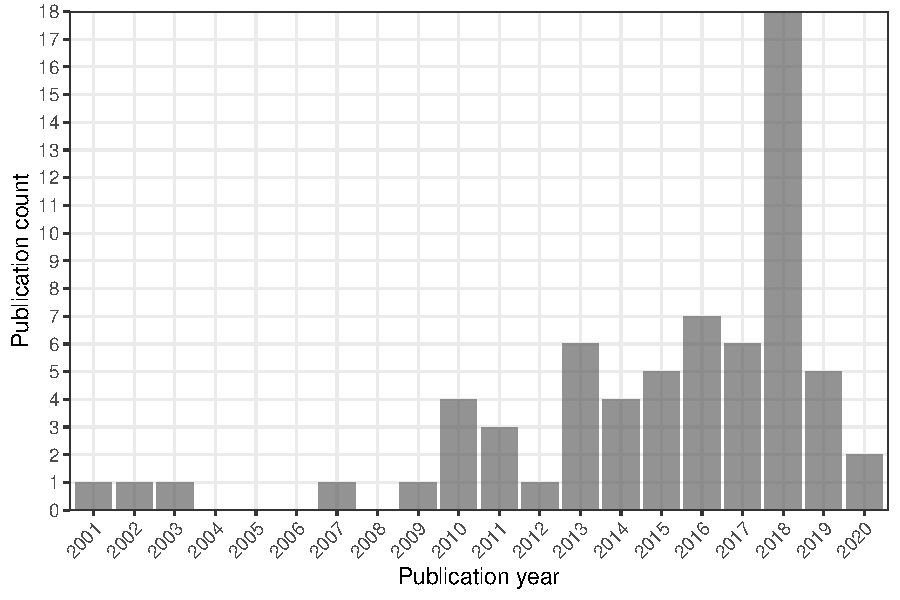
\includegraphics[width=0.85\textwidth]{survey/figures/years-publications}
		\caption{Distribution of publications across years. }
		\label{fig:years-publications}
	}
\end{figure}


\changed{
At the end of the paper collection process,
we obtained a pool of papers spanning the years 2001-2020 (June 2020).
\autoref{table:selected-primary-studies} shows
the final list of \numberOfPapers papers.
\autoref{fig:years-publications} shows the distribution of
the retrieved pool of papers across different years of publication.
Overall, we observed a generally increasing long-term trend in
the use of computer vision approaches in software engineering. 
This research area is also relatively new, 
with more than half of the papers in our pool 
published in the past five years.
Furthermore, \autoref{fig:areas-trend} depicts the cumulative number of publications 
per software engineering area across different years.
The results indicate that software testing is the area 
exhibiting the most rapid increase
in terms of the number of publications 
wherein a computer vision technique is utilized.
}




\begin{figure}
\revised{\linewidth}{
\centering
%\fbox{
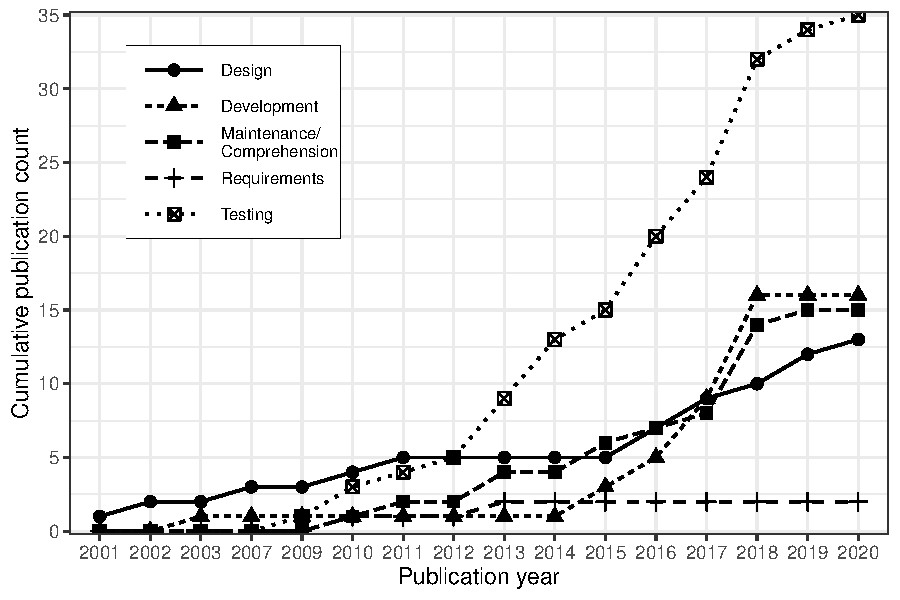
\includegraphics[width=\linewidth]{survey/figures/areas-trend-cumulative}
%}
\caption{Cumulative distribution of publications across years per SE area.
Testing is the most common area, followed by development and maintenance.} \label{fig:areas-trend} 
}
\end{figure}

\changed{
\autoref{fig:venues-publications} shows the distribution 
of the published papers across venues.
The main venues in which computer vision approaches 
for software engineering were published are 
the Conference on Human Factors in Computing Systems (CHI) with 11 papers, 
the International Conference on Software Engineering (ICSE) with nine papers, 
and the International Conference on Automated Software Engineering (ASE) with eight papers. 
The presence of traditional SE venues as well as venues from other fields (e.g. CHI) 
in \autoref{fig:venues-publications} provides some indication that 
research on the use of computer vision for software engineering tasks 
is an interdisciplinary field. 
}


\subsection{Areas, Tasks, and Platforms (RQ1)}\label{sec:rq1}

\begin{figure}%[b]
	\revised{\linewidth}{
		\centering
		%\fbox{
		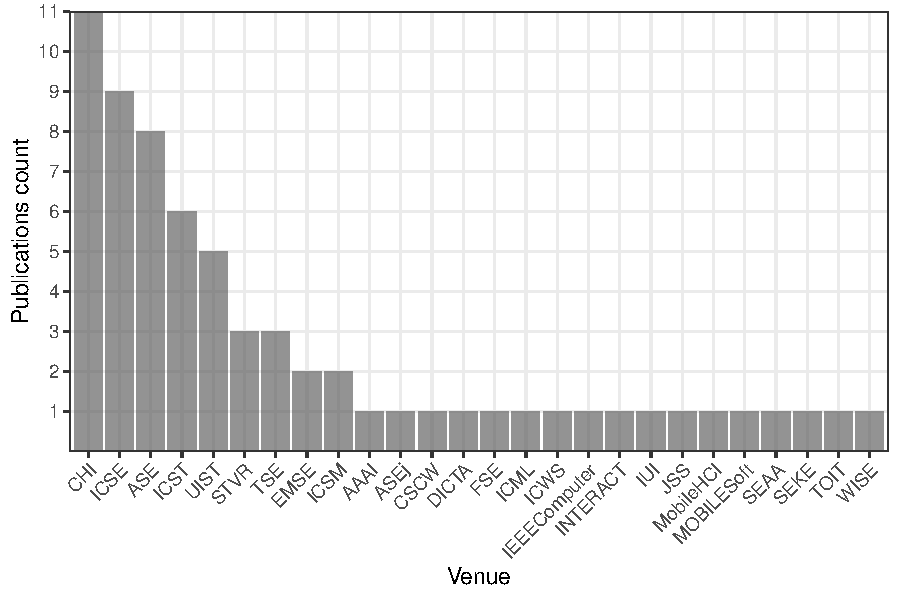
\includegraphics[width=\linewidth]{survey/figures/venues-publications}
		%}
		\caption{Distribution of the publications across venues. }\label{fig:venues-publications}
	}
\end{figure}

To study the exiting applications of visual techniques for SE,
we analyzed the selected papers to find out
which \textit{SE areas} have been explored,
for which \textit{tasks}, and on which \textit{platforms} they were used.
As defined in section \ref{sec:defs}, SE areas are high-level stages
of the software engineering life cycle,
such as requirements, testing, or development.
SE tasks are more fine-grained activities, such as unit testing or regression testing.
The platforms are the types of computing devices (e.g., desktop, mobile) 
that the analyzed software runs on. 
We further looked into the papers' discussion sections to gain insights from
the authors about other areas in which the proposed technique could potentially be applied.

\subsubsection{Software Engineering Areas and Tasks}

\autoref{fig:software-engineering-tasks}
presents the papers distribution across different SE areas and tasks.
Note that the number of papers indicated in the figure
is more than the total number of papers in the pool.
This is due to the fact that for some papers, the presented approach can be utilized for more than one task.
We now discuss more in detail the trends of \autoref{fig:software-engineering-tasks}.

\begin{figure}
    \revised{\linewidth}{
\centering
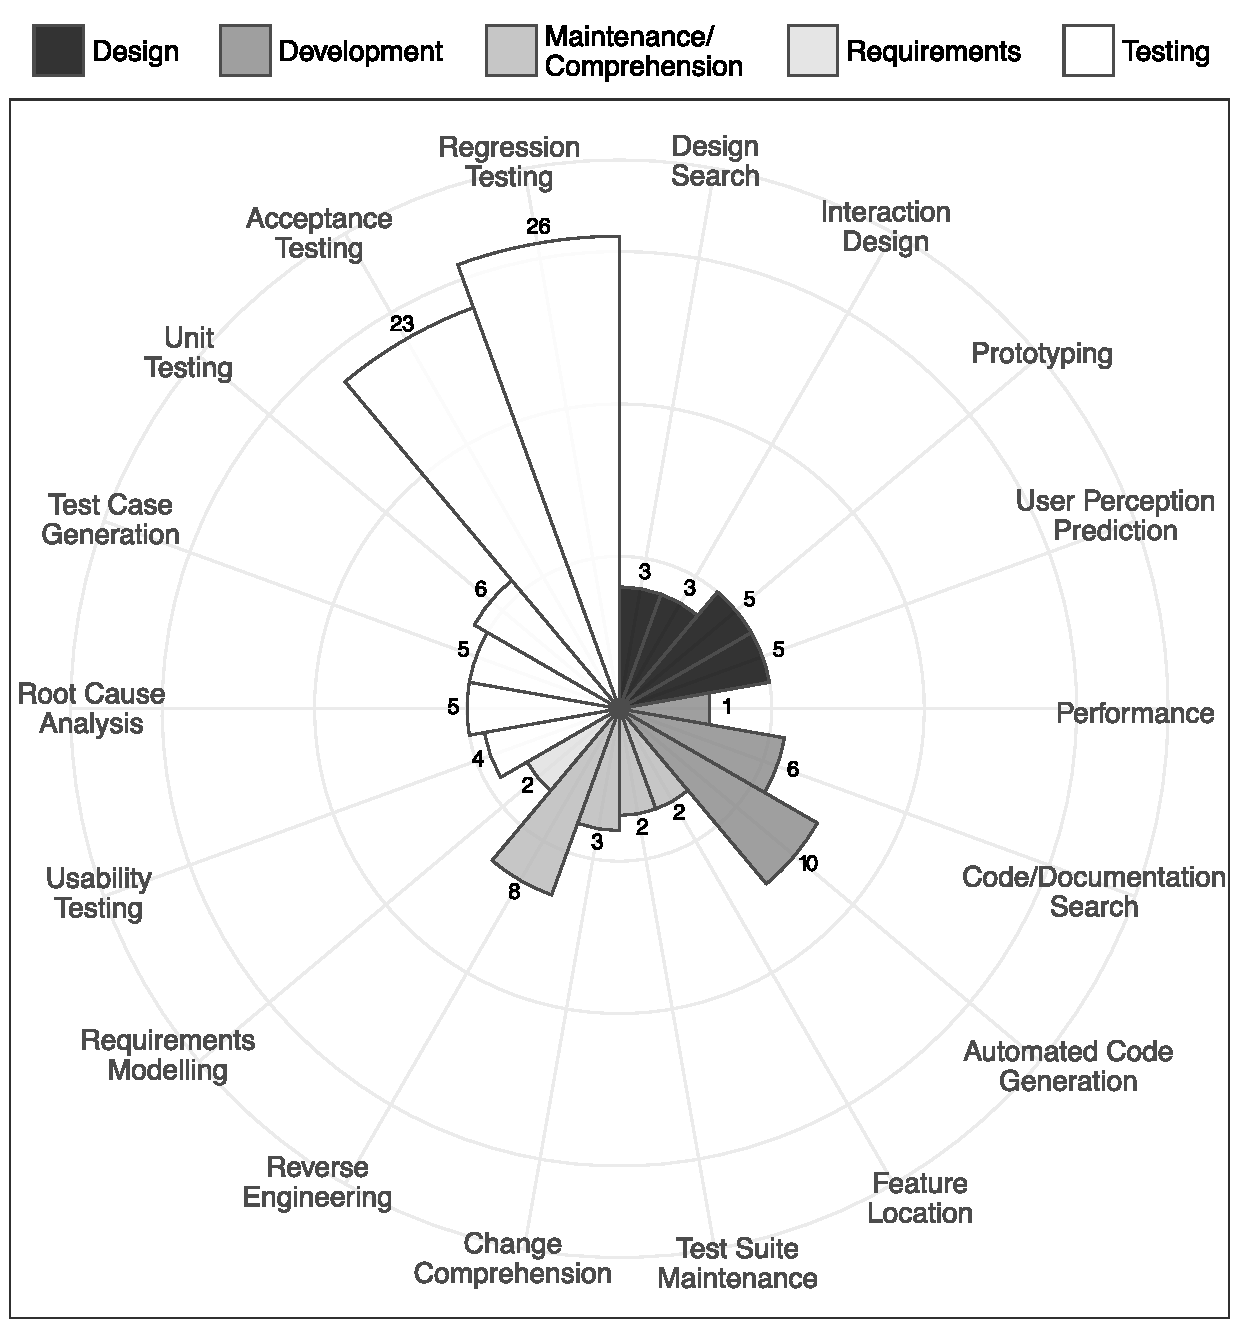
\includegraphics[width=0.8\linewidth]{survey/figures/areas}
\caption{Papers distribution across different Software Engineering Areas and Tasks}
\label{fig:software-engineering-tasks}
    }
\end{figure}


\header{Testing}
Software testing is the most common research area 
for which approaches using computer vision are proposed, 
accounting for approximately half of all collected papers.
A closer look at the publications in this area reveals interesting trends. 
\textbf{Regression Testing.} Most of the studies use visual methods to facilitate acceptance and regression testing e.g., by 
comparing visual artifacts (e.g., the GUIs) 
with each other or with respect to a given oracle.
Without adopting computer vision, developers would most 
likely need to perform some kind of manual evaluation, 
e.g., through eyeball analysis to spot deviations from 
the expected visual presentation---a daunting and error-prone task.
Apart from GUI comparisons, computer vision (CV) techniques have been also utilized 
for other software testing tasks.
%
For example,
%
\citet{Kuchta-2018-EMSE} introduce a technique for regression 
testing of PDF reader software and localizing faulty parts of PDF files.
The adopted technique exploits \textit{differential testing}, 
where the (visual) output of multiple implementations of a 
program---the PDF viewer---is compared to the same input to spot deviations.
%
In another work, \citet{Leotta-2018-STVR} propose an automated 
code migration tool for automatically converting end-to-end 
Selenium web tests to visual web tests based on 
Sikuli's~\cite{Chang-2010-CHI} image recognition capabilities.
%
\citet{Kirac-2018-JSS} provide an image comparison technique 
for black-box, regression testing of visual-output software 
used in consumer electronics.
The approach removes noise to eliminate image differences 
caused by scaling and translation, and is evaluated on the output of digital TVs.
%
\citet{canvas_icst2018} propose a technique to test 
state-free canvas elements on web pages by reverse-engineering a visual model.
This allows unit testing of the specific visual elements contained in the canvas.


\textbf{Cross-browser Testing}. A significant class of software testing techniques leveraging visual methods aims at automatically identifying \textit{cross-browser incompatibilities} (XBIs) for web 
applications~\cite{Choudhary-2010-ICSM, Choudhary-2012-ICST,
Semenenko-2013-ICSM, Choudhary-2013-ICSE, Selay-2014-DICTA, He-2016-ICWS, Xu-2018-TOIT}.
XBIs are frequently-occurring issues in web pages' 
appearance and/or behavior when the same page is viewed 
on different web browsers~\cite{Choudhary-2013-ICSE}.
Identifying such differences requires laborious human judgement,
which can be effectively reduced using an automated visual-based technique.
A recent literature review by \citet{Sabaren-2018-JCST} 
surveys the techniques proposed to tackle XBIs.

A similar problem involves using visual methods for 
\textit{root cause analysis} of presentational issues 
occurring on web pages~\cite{Mahajan-2014-ASE, Mahajan-2015-ICST,
Mahajan-2016-ICST}.
In addition to the web domain, root cause analysis 
is also used to identify rendering issues in PDF 
files~\cite{Kuchta-2018-EMSE}, as well as, the causes
of excessive energy consumption of UIs in mobile 
applications~\cite{Wan-2017-STVR}.

Several approaches attempt to automate test 
execution using visual techniques. An example 
is \textit{record-and-replay testing} where the 
screenshots of the GUI and the human tester's 
actions and inputs performed on the GUI are recorded~\cite{Chang-2010-CHI,
Alegroth-2013-ICST, Lin-2014-TSE, He-2016-ICWS} . 
Popular visual record-and-replay tools are 
Sikuli~\cite{Chang-2010-CHI} and 
JAutomate~\cite{Alegroth-2013-ICST}, which allow 
fast and easy replay of the same sequence of actions:
the tool conducts a visual search on the current 
visible contents of the screen to detect the 
widgets' locations, triggers the recorded 
actions and inputs, and finally performs a visual assertion,
comparing the observed visual outcome with the expected oracle.

Besides record-and-replay tools, test automation with 
visual analysis has been successfully applied to 
\textit{automotive software engineering}. 
\citet{Amalfitano-2014-WISE} propose a tool to automate 
the testing of the emulated vehicle information 
systems' panels.
The testers can locate visual elements on the panel 
and specify their properties; the tool allows to 
check the panel's output with respect to these 
properties at pre-defined timestamps.

\changed{
\citet{Zheng-2009-CHI}, \citet{Yuan-2020-CHI}, 
\citet{Deka-2016-UIST}, and \citet{Deka-2017-UIST} 
aim to automate the testing of \textit{aesthetics 
or usability} of web pages. 
This line of work involves building computer vision 
models that can predict whether web pages 
meet certain aesthetic requirements pertaining to 
the usability of a page (e.g. visual balance of 
white space and elements, consistent and simple 
representation of elements on a web page).
}

\citet{Patric-2016-ASE} propose an approach based 
on systematic image manipulation to \textit{automatically 
generate test input images} for regression and 
acceptance testing of an epidemiological simulation software.
The software's output on these input images is 
monitored and unexpected deviations reveal bugs or regressions in the code.

To \textit{prioritize test reports}, \citet{Feng-2016-ASE} 
use the screenshots provided by users to augment the 
existing textual test prioritization techniques for mobile applications. 
Finally, to \textit{automatically generate test cases}, 
\citet{Zhang-2017-ASE} use a visual-aided approach
that identifies strokes that testers draw on 
screenshots taken from the apps. These sketches are 
used to define test specifications (e.g., coordinates 
where a visual object should be positioned to on 
the screen), which are subsequently used to 
generate test cases automatically.

\header{Design}
\changed{
Our survey included a number of papers aiming at 
facilitating the design stage of software systems 
by means of computer vision. 
\citet{Li-2010-CHI} propose a tool to help with 
\textit{prototyping} software designs. 
Using computer vision techniques, a video 
recording of hand-drawn GUI design sketches are 
converted into a digital form. This serves as an 
interactive, clickable, documentation of the 
prototype which can be easily shared with stakeholders. 
The works of \citet{Landay-2001-IEEEComputer}, \citet{Caetano-2002-AAAI}, \citet{Coyette-2007-INTERACT}, 
and \citet{Scharf-2013-ICSE} also share the same goal of facilitating user interface prototyping by 
using computer vision to convert hand-drawn GUI 
sketches to working GUI prototypes.
}

%
\citet{Deka-2016-UIST} use a visual technique to 
learn features from mobile applications' UIs to 
create a database of UI design samples, forming 
a benchmark for \textit{ design searching}. In a 
successive work,~\citet{Deka-2017-UIST} record 
the crowed-sourced \textit{interactions} with 
the application's GUIs. This allows mining these 
interactions to incorporate them in new designs, 
and \textit{predicting users' perception} by 
their interaction with new GUIs. 
\changed{
The works of \citet{Reinecke-2016-CHI}, 
\citet{Swearngin-2019-CHI}, \citet{Wu-2020-CHI} also 
propose visual techniques to help UI designers in 
predicting the user perception of their designs.
\citet{Reinecke-2016-CHI} visually examines the color 
spectrums and arrangements in a web page, and informs 
UI designers if certain demographics (e.g. color-blind users) 
would not be able to see certain parts of their designs. 
\citet{Swearngin-2019-CHI} build a computer vision model 
that mimics users perception of ``tappability'' of 
various elements in a mobile app. Accordingly, if an app 
designer has an element that is tappable, but would not 
be perceived as tappable for the average user, the tool would 
flag such elements. \citet{Wu-2020-CHI} focuses on flagging 
animations that would be perceived (by the average user) 
as too fast, chaotic, or lacking transitions. The UI designer 
is then notified of these issues in order to mitigate them.
}

\header{Requirements Engineering}
Requirements engineering was the least explored area among all collected papers, with only two publications. This outcome is understandable since it might be due to the increasing adoption of agile development compared to the more traditional waterfall model. 
Visual techniques have been used to generate a digital form of requirement or design models (e.g., UML)
by visually processing hand-made sketches~\cite{Scharf-2013-ICSE},
or by augmenting existing requirement artifacts to make them user-tractable~\cite{Li-2010-CHI}.



\header{Comprehension and Maintenance}
Visual techniques have been used in software \textit{reverse engineering}.
The REMAUI tool~\cite{Nguyen-2015-ASE} uses computer vision techniques to reverse engineer the UI elements and their hierarchy in a mobile application
from a screenshot (or a mockup), which also allows to automatically generate the UI code.
\changed{\citet{Givens-2013-ICSE} performs a similar reverse 
engineering of the internal state of desktop applications based on visual decomposition of screenshots.}
\citet{Dixon-2011-CHI} takes this a step further by reverse engineering the hierarchy of interface components. 
\citet{canvas_icst2018} reverse engineers the state of web canvas elements from a visual screenshot of the canvas itself, which also enables testing of canvas elements. 
\changed{Deka et. al. \cite{Deka-2016-UIST}, \cite{Deka-2017-UIST} 
captures traces of user's interaction with mobile apps,
allowing the mining of user interactions from a large collection of apps.}


\changed{In another work, 
\citet{Burg-2015-UIST} use visual techniques for localizing the JavaScript code 
responsible for the implementation of a single widget 
that determines an interactive behaviour on a web application (i.e., \textit{feature location}).
\citet{Lim-2018-UIST} presents a similar tool 
but focuses on localizing the CSS implementation 
responsible for certain visual appearances.}

\citet{Stocco-2018-FSE} present a visual approach for \emph{automated test repair}; they propose a technique to repair broken web test cases by visually analyzing test executions.
Finally, Leotta et al's approach~\cite{Leotta-2018-STVR} for migrating Selenium-based web test cases to Sikuli
can help in \textit{maintaining} web tests, i.e., when it is required to convert DOM-based locators (e.g., XPath expressions)
to modern visual locators.



\header{Development}
\changed{
Visual techniques have been used for \textit{automated code generation},
simplifying the development stage of software engineering.
This includes generating UI code from mockups~\cite{Nguyen-2015-ASE, bajammal2018generating,Chen-2018-ICSE},
existing mobile apps UI code~\cite{Deka-2016-UIST, Deka-2017-UIST}, hand-made sketches~\cite{Reiss-2018-ASEj}, 
or from a video recording depicting the desired behavior~\cite{Sun-2018-ICML}.
\citet{Wu-2017-CSCW} propose a tool that automatically annotates HTML images with suitable alternative texts.

\citet{Fails-2003-CHI} present a tool that helps developers in the creation of software that processes live camera feeds, without requiring developers to have computer vision skills. \citet{Bao-2015-ICSE} proposes a similar tool that facilitates scraping of developers' screencast videos, which simplifies searching for code and documentation from video tutorials. 

\citet{Reiss-2018-ASEj} propose a technique to \textit{search code} from existing repositories
based on a given sketch, to make a compilable code from the results.
\citet{Ponzanelli-2016-ICSE} allow searching relevant code fragments
from video tutorials using visual techniques.
\citet{bajammal2018generating} generate UI component code (e.g., React, AngularJS)
from a visual analysis of a web app's mockup design.
Finally, \citet{Wan-2017-STVR} allow to spot energy pitfalls in the UIs of mobile apps,
allowing a more performance-aware UI development.
}

\subsubsection{Platforms}\label{sec:platforms}

\autoref{table:software-engineering-platforms} illustrates the results of our analysis
with respect to the platforms in which visual approaches were utilized. 
More than half of the collected papers target web and mobile platforms. 

Web and mobile applications are ubiquitous nowadays,
and their sole communication interface with users is through their GUIs.
Desktop applications, on the contrary, can often have different interfaces,
e.g., a command-line interface, or a network interface where the use of an external client software is required.
Hence, it is not surprising for visual approaches to be more utilized in web and mobile domains.
However, there are also other interesting platforms~\cite{Amalfitano-2014-WISE, Kirac-2018-JSS},
(e.g. automotive dashboards or digital TVs) where visual techniques have been successfully applied.
This indicates the potential of visual techniques in any platform where software deals with a GUI, or any artifact that is visual in nature.

\header{Summary}
This section focused on exploring the 
areas, tasks, and platforms 
where computer vision techniques have 
been proposed to address software engineering problems.
We found that software testing is the most common 
SE area where computer vision techniques
have been used. 
Within the area of software testing, 
cross-browser compatibility is the most 
frequent task that uses computer vision, and it also 
represents some the earliest works in the use of visual analysis 
for software engineering. 
Non-functional properties received little to no exploration, 
which is a research area that may potentially benefit from visual 
techniques due to the high level and semantic nature of non-functional properties. 
We also found that more than half of the collected papers 
target web or mobile platforms, as opposed to desktop.

% !TEX root =  manuscript.tex
\begin{table}
\caption{Papers distribution across different platforms }
\centering
%\small % bigger
%\small %smaller
%\setlength{\tabcolsep}{3pt}
\renewcommand{\arraystretch}{1.2}
%\revised{0.95\linewidth}{
\begin{tabular*}{0.78\linewidth}{p{2cm} p{6.5cm}}
\toprule
\textbf{Platform} & \textbf{Papers} \\																
\midrule

\text{Web} & \cite{Zheng-2009-CHI,Wu-2017-CSCW,Liang-2013-UIST,Lim-2018-UIST,Yuan-2020-CHI, Stocco-2018-FSE, Choudhary-2010-ICSM, bajammal2018generating, Li-2010-CHI, Choudhary-2012-ICST, Semenenko-2013-ICSM, Choudhary-2013-ICSE, Mahajan-2014-ASE, Selay-2014-DICTA, Burg-2015-UIST, Mahajan-2015-ICST, Hori-2015-SEKE, Mahajan-2016-ICST, He-2016-ICWS, Leotta-2018-STVR, canvas_icst2018, Xu-2018-TOIT} \\[0.5ex]

\text{Desktop} & \cite{Landay-2001-IEEEComputer, Fails-2003-CHI,Givens-2013-ICSE, Bao-2015-ICSE,Reinecke-2016-CHI,Sun-2018-ICML,Osman-2018-SEAA, Zhao-2019-ICSE, Bao-2018-TSE, Caetano-2002-AAAI, Coyette-2007-INTERACT, Dixon-2011-CHI, Dixon-2010-CHI, Chang-2010-CHI, Delamaro-2011-STVR, Scharf-2013-ICSE, Alegroth-2013-ICST, Ponzanelli-2016-ICSE, Feng-2016-ASE, Patric-2016-ASE, Bao-2017-EMSE, Reiss-2018-ASEj, Kuchta-2018-EMSE} \\[0.5ex]

\text{Mobile} & \cite{Nguyen-2015-ASE,Chen-2018-ICSE,Yu-2019-ASE,Swearngin-2019-CHI, Wu-2020-CHI, Moran-TSE-2018, Moran-ICSE-2018, Tanno-2018-ICSTW, Xiao-2019-ICSE, Moran-2018-ASE, Seifert-2011-MobileHCI, Natarajan-2018-MOBILESoft, Huang-2019-CHI, Lin-2014-TSE, Nguyen-2015-ASE, Deka-2016-UIST, Deka-2017-UIST, Wan-2017-STVR, Zhang-2017-ASE, Chen-2017-IUI} \\[0.5ex]

\text{Other} & \cite{Amalfitano-2014-WISE, Kirac-2018-JSS} \\[0.5ex]          
		
			
\bottomrule
\end{tabular*}
%}
\label{table:software-engineering-platforms}
\end{table}



% !TEX root =  manuscript.tex
\subsection{Rationale (RQ2)}

The goal of this RQ is to understand the \textit{motivations}
behind the use of visual approaches in the collected publications.
\changed{For each paper in our pool, we analyzed the paper's full text and 
noted down the rationales mentioned by the authors for using computer vision to solve the software engineering problem being tackled.
This resulted in three main categories, namely, \textit{context-driven, ease of use,} and \textit{robustness} (as will be described below). For each paper that did not explicitly mention their rationale, we analyzed the text and classified the paper to the closest rationale category. We now describe the three identified categories of rationale.}

\header{Context-driven} 
Computer vision has been utilized
because the context is intrinsically \textit{visual} in nature,
which is the case in all the papers that focused on GUIs.
Thus, it was natural for the authors to deal with a visual artifact through a computer vision technique.
More than half of the selected papers motivate the use of visual approaches
as such~\cite{Burg-2015-UIST,Feng-2016-ASE,Deka-2016-UIST,Deka-2017-UIST,canvas_icst2018,
Patric-2016-ASE,Wan-2017-STVR,Scharf-2013-ICSE,Ponzanelli-2016-ICSE,Reiss-2018-ASEj,
Bao-2017-EMSE,Nguyen-2015-ASE,Kirac-2018-JSS,Leotta-2018-STVR,Li-2010-CHI,
Amalfitano-2014-WISE,Selay-2014-DICTA,Mahajan-2015-ICST,Mahajan-2016-ICST,
He-2016-ICWS,Chen-2017-IUI,Xu-2018-TOIT,Delamaro-2011-STVR,Kuchta-2018-EMSE,
Chang-2010-CHI,Alegroth-2013-ICST}. 

For instance, \citet{Chang-2010-CHI} describe two properties of visual approaches
that make them particularly appealing for analyzing GUI-based software:
\textit{intuitiveness} and \textit{universality}.
They describe how for certain tasks, using visual artifacts---such as a GUI screenshot---
is a more spontaneous way of interaction with the software.
Due to their graphical nature, elements on the GUI can be most directly represented
by screenshots. Non-visual alternatives, such as scripting, would instead require users
to manipulate GUI elements through keywords which is arguably less intuitive. 

Furthermore, screenshots are easily accessible for all GUI-based applications.
Indeed, it is virtually always possible to take a screenshot of a GUI element,
across all applications and platforms. This can make it attractive to propose techniques 
based on analyzing visual artifacts.

\header{Ease of Use}
As a second main motivation, researchers have utilized visual approaches
because they deemed them \emph{easier} to use by end users~\cite{Choudhary-2012-ICST,
Semenenko-2013-ICSM,Choudhary-2013-ICSE,Mahajan-2014-ASE,Zhang-2017-ASE,
Choudhary-2010-ICSM,Lin-2014-TSE,Amalfitano-2014-WISE,Selay-2014-DICTA,
Mahajan-2015-ICST,Mahajan-2016-ICST,He-2016-ICWS,Chen-2017-IUI,
Xu-2018-TOIT,Delamaro-2011-STVR,Kuchta-2018-EMSE}. 
%
For instance, \citet{Zhang-2017-ASE} propose a tool that allows developers
to draw (e.g. via tablets, digital pens) simple sketches on app screenshots.
The tool then uses CV algorithms to analyze the shapes and structure of these hand
drawn sketches to decode the meaning of each sketch.
The tool then uses the sketch as a visual test spec to automatically
generate a number of GUI test suites for mobile applications.
The authors argue, and demonstrate, that providing developers with the option
of using simple hand sketches to automatically generate test cases
is a more natural and easier to use approach to create test cases compared to manually writing the test cases.


\begin{figure}
    \revised{\linewidth}{
\centering
%\fbox{
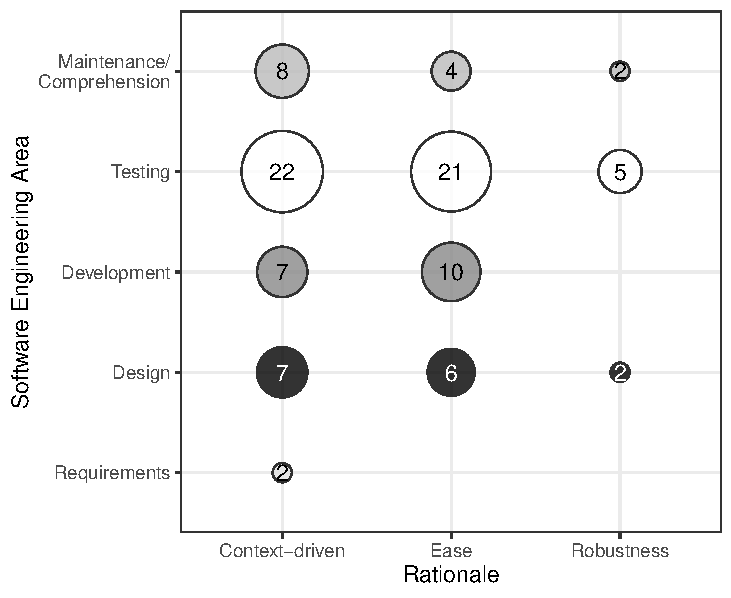
\includegraphics[width=0.8\linewidth]{survey/figures/bubbleplot-rq2.pdf}
%}
\caption{Distribution of rationales per SE area.}\label{fig:bubbleplot-rq2}
    }
\end{figure}

This viewpoint is also evident in papers targeting the detection of cross-browser
incompatibilities (XBIs)~\cite{Choudhary-2010-ICSM, Choudhary-2012-ICST, Semenenko-2013-ICSM,
Choudhary-2013-ICSE, Selay-2014-DICTA, He-2016-ICWS, Xu-2018-TOIT}.
This problem requires developers to detect visual differences between web pages within the same web application when rendered on different browsers.
This task is challenging for a number of reasons. 
First, manually performing this task, for instance through eyeballing, is neither efficient nor easy.
Hence, an automatic technique would require simulating
the reasoning that humans do while \textit{seeing and comparing} two web pages.
This can be easily simulated through a computer vision technique called \textit{image differencing}, for which a plethora of different techniques have been proposed~\cite{Choudhary-2012-ICST,
	Semenenko-2013-ICSM,Choudhary-2013-ICSE}.

However, originally, the same problem was tackled from a non-visual perspective.
First works on XBIs used well-known DOM differencing techniques as a proxy for finding visual defects. %~\cite{}. \andrea{pending cite}
The main limitation was the fact that DOM-level differences do not always
correspond to a different visual layout.
Hence, this caused such techniques to have many false positives and a low accuracy.
On the other hand, visual approaches have been proposed both as an alternative,
as well as, a complementary technique to overcome the limitations of the DOM-based approaches. 

\header{Robustness}
The concept of robustness of a visual approach concerns its capability of maintaining
its effectiveness despite minor visual changes happening in the software being analyzed.

A few papers~\cite{Chang-2010-CHI,Alegroth-2013-ICST,Tanno-2018-ICSTW} mention robustness
as rationale for choosing computer vision.
They explain that visual approaches are used because they are considered more change-tolerant than
alternative code-based techniques. In other words, according to the authors, using a code-based approach for the
same problem is likely to produce a fragile tool that would require a high maintenance cost. 

For instance, \citet{Chang-2010-CHI} describe how spatial re-arrangements of GUI components on the page
can lead to fragile test scripts, a well-known issue in web testing~\cite{Leotta-2016-JSEP}.
According to \citet{Chang-2010-CHI}, visual approaches are more robust to minor layout changes and
elements repositioning.
This viewpoint is discussed and confirmed in the paper by \citet{Alegroth-2013-ICST},
in which image recognition of GUI elements allows the development of more robust system-level automated test suites. 
A similar finding is in the paper by \citet{Stocco-2018-FSE}, in which an image processing pipeline was used to automatically trace web elements across different versions of the same web applications. Their tool \textsc{Vista} exhibited a high test repair rate during software evolution, outperforming a DOM-based test repair solution. This essentially means that in the web domain, web app GUIs exhibit less frequent changes as compared to the DOM, as acknowledged by other researchers~\cite{2015-Leotta-ICST,2016-Leotta-JSEP,Hammoudi-2016-FSE,Hammoudi-2016-ICST}.

The bubble chart of \Cref{fig:bubbleplot-rq2} shows the distribution of the rationales
in relation to the SE areas presented in \Cref{sec:rq1}.
We notice that the context-driven category dominates across all SE areas.
In the areas of requirements, design, and maintenance, visual approaches were
prevalently used because, at this stage of the software development lifecycle,
designers or requirements engineers mostly deal with visual abstractions of
(portions) the software such as GUI mockups, or UML models.
Computer vision allows the transformation of these visual artifacts to support successive SE tasks.
For example, in the work by~\citet{Zhang-2017-ASE}, annotated sketches are used
to specify test requirements and test case creation. In this case, the targeted SE
area is both requirements engineering and testing. 


\header{Summary}
In this section, 
the goal was to understand the rationales and motivations for using computer vision to
address software engineering problems.
An understanding of the rationales can help researchers
decide if their research area or topic has similar problems or challenges,
and then potentially explore using computer vision for their problem.
We identified three types of rationales by collecting and categorizing the reasons stated by the authors of each paper. There are context-driven, ease of use, and robustness.
Papers were classified as context-driven when the context of the software engineering problem itself
has dictated the use of visual approaches.
The ease of use classification was used in cases where the motivation
is not necessarily driven by the context,
but driven by the motivation of making an existing software engineering process easier to use
(e.g. has less manual work, easier to comprehend).
Finally, papers were classified as motivated by robustness whenever the motivation
is making a software engineering task more accurate or less fragile.
Out of all three categories of rationales, the context-driven category was the most common.







% !TEX root =  manuscript.tex
\subsection{Computer Vision Techniques (RQ3)}


In order to investigate how computer vision is applied, we studied:
(1)~what visual artifacts are used, generated, or extracted from the software,
and (2)~what computer vision techniques are used to process or analyze the visual artifacts.
We recall that visual artifacts are visual data (e.g.,  images) used by one or more computer vision
techniques, with the final objectives of addressing a software engineering problem.


\begin{figure}
%    \revised{0.98\linewidth}{
    \centering
    %\fbox{
    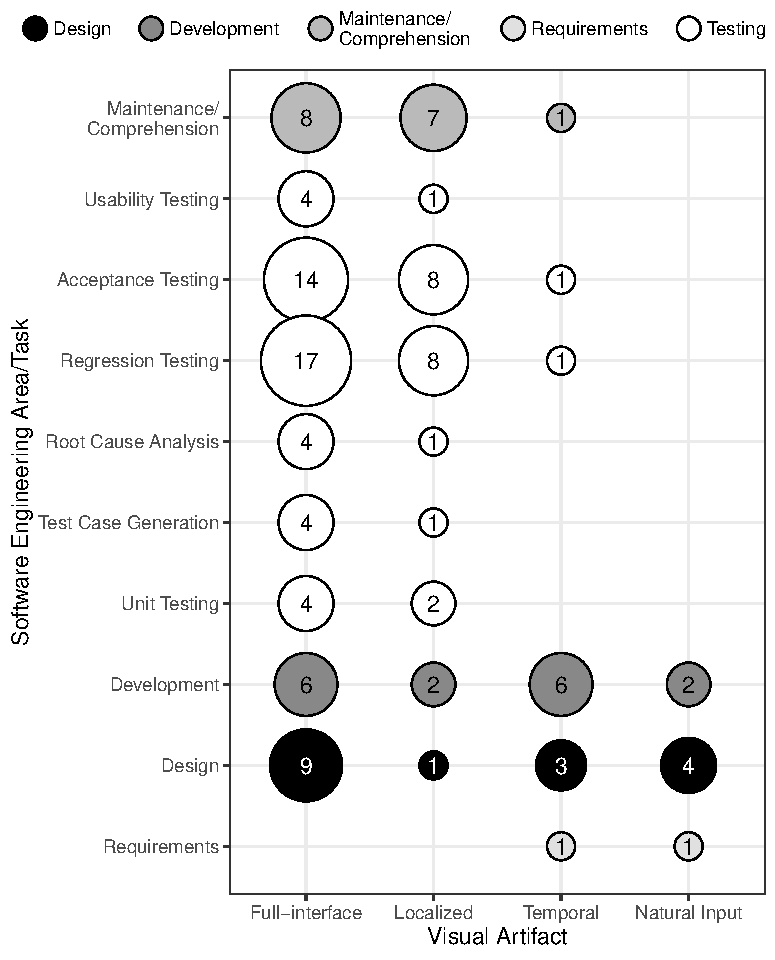
\includegraphics[width=0.8\linewidth]{survey/figures/visual-artifacts-bubble-plot}
    %}
    \caption{Distribution of visual artifacts per SE area \& task.}\label{fig-artifacts}
%    }
\end{figure}



\header{Artifact Categories}
Through our survey of the field, we classified the 
%identified a number of classes of 
visual artifacts used in the literature into four categories:
(1)~full-interface artifacts, (2)~localized artifacts,
(3)~temporal artifacts, and (4)~natural input artifacts. 
\Cref{fig-artifacts} shows the distribution of such visual artifacts 
with respect to the SE area/tasks.

The first category, \emph{full-interface visual artifacts}, typically represents
screenshots of the entire user interface of the system (whether a web browser or
desktop application, as well as other forms such as visual content of TVs and car displays)
~\cite{Choudhary-2010-ICSM,Delamaro-2011-STVR,
Choudhary-2012-ICST,Semenenko-2013-ICSM,Choudhary-2013-ICSE,Nguyen-2015-ASE,
Mahajan-2015-ICST,Deka-2016-UIST, Hori-2015-SEKE,Mahajan-2016-ICST,Feng-2016-ASE,
Patric-2016-ASE,Deka-2017-UIST,Wan-2017-STVR,He-2016-ICWS,Zhang-2017-ASE,Chen-2017-IUI,
Kirac-2018-JSS,Xu-2018-TOIT,Kuchta-2018-EMSE}.
This type of artifact simply has one large screenshot that captures the entire interface. 
This artifact has been used most commonly to capture the \textit{visual state} of the application
(regardless of the platform), and analyzed further to perform various forms of testing
(e.g., regression, acceptance, or test generation).

However, full-interface artifacts capture the visual state of the system at a coarse-grained
level of granularity, which renders them less applicable when a more detailed analysis is needed. This is because the full-interface 
captures the interface as a whole, and is therefore not very useful when the goal is more micro-scale, such as analyzing or recognizing a particular icon for instance. 
For these cases, our survey revealed another category containing  \emph{localized visual artifacts}.
In this case, visual artifacts are created at the level of a 
specific component, an area of interest, or a certain feature \cite{Chang-2010-CHI,
Alegroth-2013-ICST, Mahajan-2014-ASE, Amalfitano-2014-WISE, Selay-2014-DICTA,
Burg-2015-UIST, Leotta-2018-STVR, canvas_icst2018}.
Compared to full-interface visual artifacts, this type of artifact is more beneficial
for scenarios where analysis needs to be performed for a specific component or feature in a system. 
For instance, localized visual artifacts have been used to create a test case for a GUI
(by recording and tracking a single visual artifact for UI elements) \cite{Chang-2010-CHI},
or in debugging the rendering or capturing the behaviour of a specific HTML element in a web application~\cite{Burg-2015-UIST}. 
Had the record-and-playback used full-interface instead of localized visual artifacts, then the analysis wouldn't make much since because the test script operates at the level of elements, not entire interfaces. 

The third category that emerged is \emph{temporal artifacts}, in which the visual information
captures the \emph{dynamic behaviour} of some sequence or chain of information, states, or events
~\cite{Li-2010-CHI, Lin-2014-TSE,Ponzanelli-2016-ICSE,Bao-2017-EMSE}. 
For instance,~\citet{Bao-2017-EMSE} use a temporal artifact (a video screen recording) to construct a
tool to help researchers conducting user studies of developers' behaviours
to automatically distill and transcribe their actions, inputs, and event sequences
by capturing a video screen recording of their work session.

Finally, 
the last identified category is \emph{natural input artifacts}.
These artifacts capture a natural representation or interaction with a human user.
The only example of this artifact that we found in the collected literature are
hand-sketches~\cite{Scharf-2013-ICSE, Reiss-2018-ASEj}.
This type of artifact provides a number of benefits:
(1)~it provides a more intuitive and natural way for software engineers to interact with,
    design, develop, or test their software, and
(2)~it allows a broad degree of freedom in capturing user input,
    which can be useful when modelling or analyzing multi-variable complex systems.



% !TEX root =  manuscript.tex

%\begin{table*}[t!]
\begin{sidewaystable}
    \caption{Major computer vision algorithms used in the collected papers.}
    \centering
    %\renewcommand{\arraystretch}{1.2}
	\setlength{\tabcolsep}{9pt}
%	\revised{\textwidth}{
    \begin{tabular}{l l p{5.5cm} p{3cm}}
        \toprule
        \textbf{Visual Technique}	& \textbf{Algorithm}	& \textbf{Description}		& \textbf{Utilized in} \\
        \midrule
        \multirow{9}{*}{Differential} 	
        		& \multirow{2}{*}{Image diff}
        													& A processing method whose output is a function of the 
        														difference between a pair of input images (e.g. PID--Perceptual Image Differencing~\cite{ref:PID},
																PHash--Perceptual Hashing~\cite{ref:PHash}).
       	 		& \cite{Selay-2014-DICTA, Delamaro-2011-STVR, Deka-2016-UIST, Kuchta-2018-EMSE, Zhao-2019-ICSE,Liang-2013-UIST,Lim-2018-UIST,Bao-2015-ICSE,  Choudhary-2010-ICSM, Li-2010-CHI, Mahajan-2014-ASE, Burg-2015-UIST, Mahajan-2015-ICST, Ponzanelli-2016-ICSE, Mahajan-2016-ICST, Deka-2017-UIST, Bao-2017-EMSE, Chen-2017-IUI, Kirac-2018-JSS, Xu-2018-TOIT, Moran-ICSE-2018, Moran-2018-ASE}   \\
		& & & \\
        	 																				
                & \multirow{2}{*}{Probability distribution distance}
                                   							& Measuring the distance between \emph{distributions} of pixels 
                                   							in a pair of images (e.g. $\chi^2$ distribution distance). 
                & \cite{Choudhary-2010-ICSM, Choudhary-2012-ICST, Choudhary-2013-ICSE, Lin-2014-TSE,Hori-2015-SEKE, Feng-2016-ASE,He-2016-ICWS, Xu-2018-TOIT, bajammal2018generating, Moran-2018-ASE} \\
                                   							
		\midrule
        \multirow{8}{*}{Transformational}
        		& \multirow{2}{*}{Color/Spatial transformation}
        													& Applying a transformation matrix to the spatial or color-space of one or more images, or transforming spatial regions into abstract data.
				& \cite{Dixon-2010-CHI, Reiss-2018-ASEj,    Fails-2003-CHI, Zheng-2009-CHI,Givens-2013-ICSE,Bao-2015-ICSE,Reinecke-2016-CHI, Caetano-2002-AAAI, Coyette-2007-INTERACT, Dixon-2011-CHI, Seifert-2011-MobileHCI,  Natarajan-2018-MOBILESoft, Osman-2018-SEAA, Huang-2019-CHI, Li-2010-CHI, Patric-2016-ASE, Wan-2017-STVR, Kirac-2018-JSS, canvas_icst2018, Moran-TSE-2018, Moran-ICSE-2018, Xiao-2019-ICSE} \\

		& & & \\
                & \multirow{2}{*}{Optical character recognition}
                                    						& Recognizing images of strings and converting them 
                                    						into textual data.
                & 
%                \multirow{2}{*}{
                	\cite{Yu-2019-ASE, Chang-2010-CHI, Amalfitano-2014-WISE, Nguyen-2015-ASE, Ponzanelli-2016-ICSE, Bao-2018-TSE, Tanno-2018-ICSTW, Xiao-2019-ICSE}
%                } 
            \\
		\midrule				
            	& Template matching		& Finding where an image is located within another image. 
				& \cite{Alegroth-2013-ICST, Dixon-2010-CHI, Bao-2018-TSE, Givens-2013-ICSE, Yu-2019-ASE, Chang-2010-CHI, Semenenko-2013-ICSM, Lin-2014-TSE, Bao-2017-EMSE, Chen-2017-IUI, Leotta-2018-STVR, Stocco-2018-FSE, Tanno-2018-ICSTW} \\
		Search							&   &   &   \\
				& Machine learning		& Finding closest visual matches or categories based on learning patterns in visual data. 
				& \cite{Scharf-2013-ICSE,  Landay-2001-IEEEComputer,  Deka-2016-UIST, Zhang-2017-ASE, Reiss-2018-ASEj,       Wu-2017-CSCW,Chen-2018-ICSE,Sun-2018-ICML,Zhao-2019-ICSE,Swearngin-2019-CHI,Yuan-2020-CHI,Wu-2020-CHI,Fails-2003-CHI} \\
        \bottomrule
    \end{tabular}
		\label{tbl:cv-algorithms}
%	}
%\end{table*}
\end{sidewaystable}

\header{Visual Techniques Taxonomy}

\begin{figure}
    \centering
    %\fbox{
    
\includegraphics[width=\linewidth]{survey/figures/taxonomy}
    %}
    \caption{Synthesized taxonomy of visual techniques.}
    \label{fig:taxonomy-rq3}
\end{figure}

In this section, we describe a taxonomy of visual techniques.
The taxonomy was synthesized from the pool of papers we collected 
in this survey. 
This taxonomy has not been used elsewhere, since 
there are no existing surveys on the use of computer 
vision techniques in software engineering.
For each paper, we analyzed the text and 
noted down the computer vision algorithms utilized by the authors 
to solve the software engineering problem being tackled.
After conducting this process over all collected papers, 
we grouped the algorithms and identified three main patterns of algorithms,
which are then collected in a taxonomy.
We built the taxonomy in an iterative manner,
where a new taxonomy category is defined if a certain computer vision algorithm 
can not be classified under any of the existing categories.

\autoref{fig:taxonomy-rq3} shows the resulting taxonomy.
As shown in the figure, we identified three main categories
of visual techniques used in software engineering research:
(1)~differential, (2)~transformational, and (3)~search techniques.
Each technique has sub-categories of algorithms, which will be described in Section \ref{sec:CV-algos}.


\emph{Differential techniques}: a visual analysis process that takes  two or more visual artifacts as input, and outputs their differences~\cite{Delamaro-2011-STVR,Choudhary-2012-ICST,
Choudhary-2010-ICSM,Alegroth-2013-ICST,Choudhary-2013-ICSE,Lin-2014-TSE,Mahajan-2014-ASE,
Amalfitano-2014-WISE,Selay-2014-DICTA,Burg-2015-UIST,Mahajan-2015-ICST,Hori-2015-SEKE,
Mahajan-2016-ICST,Feng-2016-ASE,Deka-2017-UIST,He-2016-ICWS,Kirac-2018-JSS,Xu-2018-TOIT}. 
The nature of these differences is typically case-specific and often targets a specific
feature that the paper is considering.
Differential techniques are commonly used in situations where a comparison of different aspects,
options, or versions of the software is desired.
For instance, they have been widely utilized for cross-browser testing
~\cite{Xu-2018-TOIT, Choudhary-2010-ICSM, He-2016-ICWS, Choudhary-2012-ICST, Selay-2014-DICTA},
where the goal is to check for any differences between two or more browsers in the way they 
render a web app.

The second category, \emph{transformational techniques}, achieve a specific software engineering task
by transforming the visual artifact into a more abstract type of information
~\cite{Scharf-2013-ICSE,Semenenko-2013-ICSM,Nguyen-2015-ASE,Deka-2016-UIST,Ponzanelli-2016-ICSE,
Patric-2016-ASE,Wan-2017-STVR,Bao-2017-EMSE,Zhang-2017-ASE,Reiss-2018-ASEj,canvas_icst2018,Kuchta-2018-EMSE}.
This transformation is typically case-specific, as the higher-level abstract information
is used to solve the specific instance of problems addressed in the paper.
For instance, this approach has been used to allow manual hand-drawn strokes as a method to specify
test executions and requirements~\cite{Scharf-2013-ICSE},
where transformational techniques are applied on hand-drawn stroke instances to extract testing
instructions and assertions from the strokes, and finally generate a working test case.

Finally, the third category is \emph{search techniques}~\cite{Chang-2010-CHI, Li-2010-CHI,Chen-2017-IUI,Leotta-2018-STVR}.
In this case, a visual artifact is used as a key to find information within a larger set of visual artifacts.
A popular example of this approach is visual record-and-playback tools such as Sikuli~\cite{Chang-2010-CHI}.
These tools first record component visual artifacts for every GUI element clicked or interacted with
by a developer or user, and then, in the playback phase, a visual search method is employed to locate
the element on screen to perform the recorded action (e.g., click).

\begin{figure}
%    \revised{\linewidth}{
    \centering
    %\fbox{
    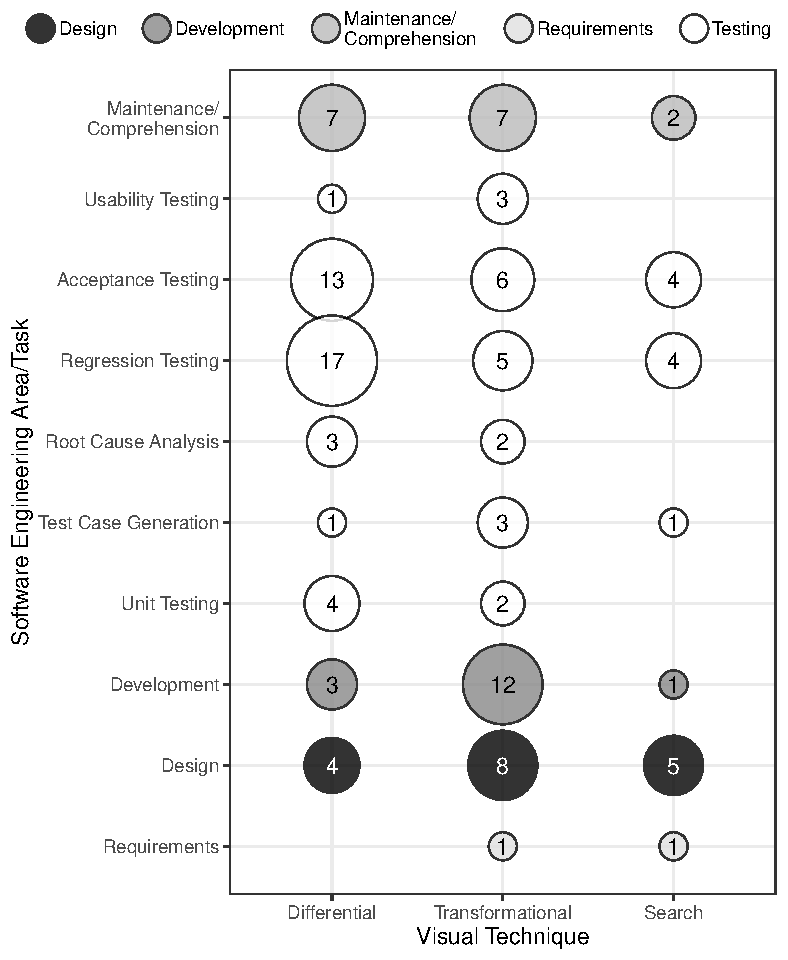
\includegraphics[width=0.8\linewidth]{survey/figures/bubbleplot-rq3}
    %}
    \caption{Distribution of visual techniques per SE area \& task.}\label{fig:bubbleplot-rq3}
%    }
\end{figure}


In order to have a better insight on the use of different 
categories of visual techniques,
the bubble plot of \autoref{fig:bubbleplot-rq3} shows their distribution over the various SE areas.
In the plot, software testing has a finer-grained granularity
since it is by far the most represented area in our final pool of papers.
We make a number of observations from the plot.
First, we notice that transformational techniques are more uniformly represented across all SE areas and tasks.
This is a somewhat expected result 
since transformational techniques are generic enough to be used 
on their own, or in addition to other techniques as pre- or post-processing steps. 
Next, we also notice that differential techniques were relatively common in testing tasks.
For instance, regression and acceptance testing greatly benefit from differential techniques,
since they are very well aligned towards detecting differences and therefore suitable for indicating regression faults.

    
\subsubsection{Computer Vision Algorithms}
\label{sec:CV-algos}

In addition to the preceding analysis of the high-level categories of visual techniques,
we also examine the specific computer vision algorithms used in the collected pool of papers.
\autoref{tbl:cv-algorithms} shows the algorithms that have emerged from our analysis.
We now describe each of the identified algorithms.

\header{Image Diff}
In these CV algorithms,
a pair of images is taken as input
and the output is defined as a function of the \emph{difference}  between the pair.
Various instances of these algorithms differ in their choice of the output function.
For instance, the most common variation uses the raw absolute difference as the output value~\cite{Choudhary-2010-ICSM,Li-2010-CHI,Mahajan-2014-ASE,Ponzanelli-2016-ICSE,
Deka-2017-UIST,Bao-2017-EMSE,Chen-2017-IUI,Kirac-2018-JSS,Moran-ICSE-2018},
where it is useful for faithfully detecting any \textit{pixel-level} difference.
Another variation adopts a more relaxed approach
where the output function captures only \emph{perceivable} differences by humans
using algorithms such as PID (Perceptual Image Differencing)~\cite{ref:PID},
PHash (Perceptual Hashing)~\cite{ref:PHash},
and Structural Similarity Index (SSIM)~\cite{ref:SSIM},
which aim to reduce false positives by mimicking human perception.
These techniques were utilized in~\cite{Mahajan-2015-ICST,Mahajan-2016-ICST,
Xu-2018-TOIT,Moran-ICSE-2018,Moran-2018-ASE,Burg-2015-UIST}. 

\header{Probability Distribution Distance}
These algorithms quantify distances in \emph{populations} of pixels,
as opposed to a pixel-wise comparison.
The goal here is to measure how similar two given distributions are,
such as image \emph{histograms}~\cite{223129} which give the distribution of pixels in an image.
This is then used to establish whether the two
distributions of pixels can be assumed to represent similar visual
information.
The $\chi^2$ histogram distance (for both coloured and grayscale data)
is by far the most commonly used distribution distance
in our pool of papers~\cite{Choudhary-2012-ICST,Choudhary-2013-ICSE,
Hori-2015-SEKE,Feng-2016-ASE,He-2016-ICWS, Moran-2018-ASE},
as it is readily available in many implementations
and provides a simple and effective approach for the needed quantification of distance.

\header{Color/Spatial Transformation}
These algorithms perform a transformation
of the spatial or color-space of one or more images~\cite{Li-2010-CHI,Patric-2016-ASE,Wan-2017-STVR,Kirac-2018-JSS,
canvas_icst2018,Moran-TSE-2018,Moran-ICSE-2018,Xiao-2019-ICSE}.
This constitutes applying a 2D or 3D transformation matrix
on the desired geometric space (e.g., a rearrangement of color-space).
This class of algorithms has been used in our pool of papers
to perform tasks such as extracting structure from images,
aligning images, and various forms of thresholding to extract content.

\header{Optical Character Recognition (OCR)}
OCR algorithms use a series of computer vision analyses
to recognize strings in images.
Once the string is recognized, another sequence of steps
converts each character in the image to textual data.
We found multiple papers in our pool (e.g., \cite{Chang-2010-CHI, Amalfitano-2014-WISE,
Nguyen-2015-ASE, Ponzanelli-2016-ICSE, Bao-2018-TSE, Tanno-2018-ICSTW, Xiao-2019-ICSE})
which have used OCR for tasks such as checking GUI component labels and
generating component labels from mockups/screenshots.

\header{Template Matching}
Another major class of CV algorithms used in the papers is template matching.
Here, one image is searched within another image or set of images.
That is, a visual scan is performed to find a template image (hence the name)
in a larger image or set of images.
Several papers in our pool~\cite{Chang-2010-CHI, Semenenko-2013-ICSM,
	Lin-2014-TSE, Bao-2017-EMSE, Chen-2017-IUI, Leotta-2018-STVR,
	Stocco-2018-FSE, Tanno-2018-ICSTW} have used this approach
to achieve tasks such as locating and finding coordinates of components and
checking the presence/absence of components or certain features within
a set of GUIs. While it may appear that template matching 
is related to the OCR class of techniques, it is actually different. 
This is because OCR converts an image to a string, while template matching finds the location of a given image within another image. 

\header{Machine Learning}
Machine learning has also been used by a few papers in our pool.
For instance, \emph{decision trees} were used for classifying web pages
in cross-browser testing~\cite{Choudhary-2012-ICST,Semenenko-2013-ICSM}.
\emph{Convolutional neural networks} (CNNs) were also used
to analyze GUIs and their content~\cite{Moran-TSE-2018,Semenenko-2013-ICSM}.
Furthermore, scale- and transformation-invariant features
(e.g.,  SURF--Speeded-Up Robust Features~\cite{ref:SURF}, Wavelets~\cite{ref:wavelet}),
which are basically features aiming at analyzing image structure and content,
were used to classify and detect GUI elements
~\cite{Xiao-2019-ICSE,Stocco-2018-FSE,Kuchta-2018-EMSE,Bao-2017-EMSE}.


% !TEX root =  manuscript.tex
\begin{table}%[t]
    \caption{Open-source and industrial computer vision tools and libraries utilized by papers in the pool. }
%     \andrea{This table was here in the previous revision as well. Highlight that the second part of the table are the industrial solutions the reviewer's asked for}}
    \centering
    %\small % bigger
    %\small %smaller
    \setlength{\tabcolsep}{8pt}
    \renewcommand{\arraystretch}{1.2}

%\revised{0.48\textwidth}{
    \begin{tabular}{p{2cm} p{6cm} p{3cm}}
    \toprule
    \textbf{Name} & \textbf{Scope} & \textbf{Utilized in} \\																
    \midrule
    
    OpenCV %~\cite{lib:opencv} 
            & provides data structures and algorithms for a wide variety of advanced computer vision processing 
            & \cite{Tanno-2018-ICSTW, Givens-2013-ICSE, Bao-2015-ICSE, Zhao-2019-ICSE, Moran-TSE-2018, Xiao-2019-ICSE,  Bao-2017-EMSE,   Feng-2016-ASE,  Stocco-2018-FSE, Mahajan-2016-ICST, Nguyen-2015-ASE, Leotta-2018-STVR, Mahajan-2015-ICST, Chang-2010-CHI,Choudhary-2010-ICSM, Choudhary-2012-ICST, Choudhary-2013-ICSE, Lin-2014-TSE} \\[0.5ex]
    Tesseract%~\cite{lib:abbyfinereader} 
            & extensible and modular open-source optical character recognition (OCR) engine
            & \cite{Nguyen-2015-ASE, Ponzanelli-2016-ICSE,Moran-TSE-2018,Yu-2019-ASE} \\[0.5ex]    
    FineReader%~\cite{lib:abbyfinereader} 
            & comprehensive OCR engine that includes relevant pre/post-processing steps and formats 
            & \cite{Bao-2018-TSE} \\[0.5ex]
    BoofCV%~\cite{lib:boofcv} 
            & performance-oriented library that focuses on real-time processing 
            & \cite{Ponzanelli-2016-ICSE} \\[0.5ex]
    ImageMagick%~\cite{lib:imagemagick} 
            & simple and easy to use tool and library for basic image transformations and analysis of color 
            & \cite{Mahajan-2014-ASE} \\[0.5ex]

    \midrule
    ITK (Insight ToolKit)%~\cite{lib:itk} 
    & specialized in image and coordinates matching, with comprehensive support for high-dimensional data & N/A \\[0.5ex]
    VLFeat%~\cite{lib:vlfeat} 
    & geared towards feature extraction, covering a large set of feature descriptors & N/A \\[0.5ex]
    ImageJ%~\cite{lib:imagej} 
    & a modular tool and library with an extensive number of plugins for various image analysis tasks & N/A \\[0.5ex]
    Amazon Rekognition, Google Vision AI, Azure CV
    %~\cite{lib:awscv, lib:googcv, lib:azurecv} 
    & cloud-based tools with a large number of pretrained analysis and recognition models & N/A \\[0.5ex]
    
    \bottomrule
    \end{tabular}
%    }
    \label{table:cvlibs}
    \end{table}



\header{Libraries and Tools}

% \revised{0.48\textwidth}{
\changed{
We also investigated what industrial or open-source 
libraries and tools were used by the papers in their 
implementation of computer vision techniques. 
\autoref{table:cvlibs} shows a list of the CV tools 
or libraries that have been used by the papers in our pool. 
The first column reports the name of the tool or library. 
The second column describes the scope of the library, 
and the last column shows the paper(s) that utilize 
a certain library to implement their CV analysis or processing. 
Papers that do not state which library or tool they used are not 
included in the table, and therefore the number of papers 
in the table is smaller than the total pool.
For the sake of completeness, we also included other 
CV tools and libraries that have not been used by 
any of the papers in our pool, which are marked 
by the ``N/A'' (not applicable) value in the last column. 
These tools were included in order to present the software 
engineering research community with an easy access to a list of 
other computer vision tools that they might find helpful to use. 
Due to the absence of queryable databases in 
which computer vision tools are listed, we resorted 
to manual search engine queries to find computer 
vision tools or libraries other than those already 
used by our pool. The queries we used were of the 
form ``alternative (libraries or tools) to X'', 
where X is one of the libraries already in our pool. %\andrea{vague}

The most commonly used library is \emph{OpenCV}.
\footnote{https://opencv.org} This library has 
implementations for a large number of CV algorithms, 
including all the algorithms we report in this 
survey (Section \ref{sec:CV-algos}). It was first 
released in 2000, and is still in active development. 
Other than OpenCV, a few other libraries were used 
by only a handful of papers. 
\emph{ImageMagick}\footnote{https://imagemagick.org/} 
is a simple and easy to use library offering basic 
quick image manipulations (e.g.,  resize, rotate).  
\emph{ImageJ}\footnote{https://imagej.net} is also 
quite similar in features and scope.
\emph{Tesseract}\footnote{https://github.com/tesseract-ocr/tesseract} 
is a popular open-source library that is modular and extensible, 
with support for more than 100 languages.
\emph{Abby FineReader}\footnote{https://abbyy.com/} is 
a commercial library that focuses specifically on 
OCR and includes many related preprocessing/postprocessing 
algorithms, as well as various file formats.
\emph{BoofCV}\footnote{http://boofcv.org} focuses 
on performance-tuned algorithms and is geared 
towards cases where real-time response is priority.
\emph{ITK}\footnote{https://itk.org/} focuses on 
high-dimensional visual data often present 
statistics and science, and also has extensive 
image coordinates matching algorithms that 
might be beneficial in a number of image 
matching applications. 
\emph{VLFeat}\footnote{https://vlfeat.org/} is 
geared towards implementing a wide variety of 
feature extraction and matching algorithms, 
enabling applications in image search or transformation.
Finally, there are cloud-based tools offered by 
major cloud hosting providers (e.g. Amazon Web 
Services, Google Cloud Platform, Microsoft Azure). 
The defining feature of these services is their 
cloud nature and the availability of many 
pre-trained computer vision models for various 
visual tasks, such as content tagging and 
visual path analysis. 
}

\begin{table}[]		\scriptsize
	\caption{Summary of the analysis approaches for the targeted research problems.}
	\begin{tabular}{lll}
		
		\textbf{Non-functional Property} & \textbf{Research Problems}                                                                        & \textbf{Approach}                                                                                                                                                                                                                                         \\
		\hline \\
		
		Accessibility           & \begin{tabular}[c]{@{}l@{}}- testing semantic roles\\ - repairing form labels\end{tabular} & \begin{tabular}[c]{p{4.5cm}}
			- identifying page regions, then computing and sorting ratios of visual locations, areas, visual size variance, and neural network classification. 
			\\ - abstracting form elements, then combining visual layout (relative spacing) with visual prominence (weight, size, color), and finally  optimizing label assignment
		\end{tabular} \\
		%		\begin{tabular}[c]{p{4.5cm}}Existing works perform syntax checks. Semantic roles and form labels are not tested or repaired. The work in this dissertation tests roles and repairs labels by analyzing visual cues from the page.\end{tabular} \\
		
		\\
		\hline \\
		
		Maintainability         & \begin{tabular}[c]{@{}l@{}}- generating reusable \\ components\end{tabular}                & 
		\begin{tabular}[c]{p{4.5cm}}- visual normalization of the page based on 
			element location, dimensions, and type, followed by histogram clustering \end{tabular} \\
		
		
		\\
		\hline \\
		
		Testability             & - testing canvas elements                                                                  & \begin{tabular}[c]{p{4.5cm}}- detecting and isolating object boundaries, then identifying their shapes, dimensions, colors, and hierarchy \end{tabular}                              \\
		
		
	\end{tabular}
	\label{tbl:summary-techniques}
\end{table}

\header{Overview of the proposed techniques}
In this dissertation, we propose a number of visual analysis techniques 
to improve the non-functional properties of testability, accessibility, and 
maintainability. An introduction to these properties and the motivation for 
exploring them is discussed in \Cref{chp:intro}. In \Cref{tbl:summary-techniques}, 
we show an overview of the approaches used, which are presented here only in a high-level and will be discussed in detail in their relevant chapters. 
While existing works are mostly based on using entire images, say, for diffing or searching, the techniques in this dissertation operate at a fine-grained level of analysis. By fine-grained we mean that the analysis focuses on very specific visual features that may potentially be helpful in addressing the research problem. 
For instance, when we analyze canvas elements, 
one fine-grained aspect that is used is extracting and identifying the boundaries 
of each object, in order to help detect the type of each object and express it in the 
DOM. Accordingly, the approaches are based on identifying what fine-grained features should be selected, where should they be collected from, how would they be combined,  
and how to analyze them to address the research problem. Each of these aspects 
is problem specific and need to be explored and determined according to the objective and constraints of the problem. 

\header{Summary}
The goal of this subsection was to explore what computer vision techniques
were used and what visual artifacts were extracted from the software.
To this end, we identified four categories of artifacts.
The first category, full-interface artifacts, represents cases
where the entire visual content of a software is used (e.g.,  entire desktop interface, entire console).
The second category is localized artifacts, where only a specific module
or component of the software is captured visually. 
Third, temporal artifacts capture the dynamic behavior of the states or events in a software. Finally, natural input artifacts capture natural forms of input by humans (e.g.,  hand sketches).
%
Visual artifacts are then processed by one or more of three visual techniques.
The first category, differential techniques, are based on various forms of contrasting two or more visual artifacts and using the differences to solve a software engineering problem.
The second category, transformational techniques, rely on transforming the visual artifact into a more abstract data structure on which further analysis can be conducted.
Finally, in search techniques, a visual artifact is used as a key to find information within a larger set of visual artifacts.

\autoref{tbl:cv-algorithms} shows the major computer vision algorithms used in the collected papers.
The visual technique column describes the high-level goal of what the algorithm is trying to achieve visually.
The algorithm column lists the specific algorithms that were used to achieve the task.
For instance, when papers wanted to do a differential examination of visual artifacts, the two computer vision approaches that were used were image diffing and distribution distances.



% !TEX root =  manuscript.tex
\subsection{Evaluation and Challenges (RQ4)}


\header{Evaluation Methods}

We systematically studied the selected papers to 
understand the most common methods used for 
evaluating the proposed visual approaches.
\Cref{table:evaluation-techniques} (Evaluation 
Methods) depicts the results: the evaluation 
methods presented are not necessarily disjoint,
since one technique can for instance be evaluated 
with respect to its performance (i.e., running time), 
and its accuracy calculated by the judgment of human participants.

In more than half of the works (53\%), the 
evaluation methods were performed using 
wide-spread effectiveness assessment 
measures such as precision and recall
~\cite{Choudhary-2010-ICSM, Choudhary-2012-ICST, 
Choudhary-2013-ICSE, Lin-2014-TSE, Nguyen-2015-ASE, 
Mahajan-2015-ICST, Hori-2015-SEKE, Feng-2016-ASE, 
Patric-2016-ASE, Wan-2017-STVR, He-2016-ICWS, 
Bao-2017-EMSE, Chen-2017-IUI, Reiss-2018-ASEj, 
Kirac-2018-JSS, canvas_icst2018, Kuchta-2018-EMSE, 
Xu-2018-TOIT}.

Another significant body of work measured 
the manual effort saved by the visual approach 
with respect to the humanly performed 
task~\cite{Delamaro-2011-STVR, Li-2010-CHI, 
Li-2010-CHI, Semenenko-2013-ICSM, Mahajan-2015-ICST, 
Feng-2016-ASE, Chen-2017-IUI, Leotta-2018-STVR, 
Reiss-2018-ASEj}. 
Moreover, several works also evaluated the 
performance of the proposed approaches, 
usually measuring the running time on common 
developer platforms (i.e., mid-level 
notebooks)~\cite{Nguyen-2015-ASE, Selay-2014-DICTA, 
Hori-2015-SEKE, Patric-2016-ASE, Wan-2017-STVR, 
Bao-2017-EMSE, Reiss-2018-ASEj, Kirac-2018-JSS}.

Performance is potentially considered as 
important as the accuracy because image analysis 
techniques are deemed as being computationally 
expensive. Thus, their application and use must 
carefully evaluate the overhead imposed by 
these visual approaches over the most general 
SE tool being developed. Initially, this might 
not favor their adoption if compared to other 
less computationally-intensive approaches.
However, the authors report that the time 
taken by their proposed techniques are all 
reasonable in common processing environments, 
suggesting that execution time should not be 
considered as a deterrent decision criterion when 
adopting a visual approach to support a SE task.

In several works, the human expertise was used to 
assess the output of the visual 
techniques~\cite{Mahajan-2015-ICST, Hori-2015-SEKE, 
Mahajan-2016-ICST, Kuchta-2018-EMSE, Xu-2018-TOIT, 
Ponzanelli-2016-ICSE, Choudhary-2010-ICSM, 
Choudhary-2012-ICST, Choudhary-2013-ICSE}.
As an example, \citet{Mahajan-2015-ICST} examine 
the efficacy of WebSee (a tool that identifies 
presentational failures in HTML pages)
through manual investigation of its output
when it is executed on 253 automatically-generated 
test cases.
This is done to see whether WebSee is able to 
correctly identify the faulty HTML elements
seeded when generating the test cases.
While we were expecting more human judgment 
involved in the evaluation of the selected papers, 
its application depends largely on the context 
and the problem being solved. 

Four works do not propose a quantitative empirical 
evaluation of the proposed technique, but 
rather present them by means of use cases.
A closer look at these publications revealed 
that two of them are short papers~\cite{Alegroth-2013-ICST, Scharf-2013-ICSE},
where having a more thorough evaluation is not 
mandatory. 
The other two papers~\cite{Burg-2015-UIST, 
Deka-2016-UIST} were published at the ACM Symposium 
on User Interface Software and Technology (UIST), 
in which use case demonstrations appear to be more frequent.
Four works included an industrial 
evaluation~\cite{Li-2010-CHI, Mahajan-2015-ICST, 
Amalfitano-2014-WISE, Kuchta-2018-EMSE} where the work is evaluated 
through feedback or measurements in an industrial setting.

% !TEX root =  manuscript.tex
\begin{table}
\caption{Evaluation methods and challenges.}
\centering
\setlength{\tabcolsep}{8pt}
%\renewcommand{\arraystretch}{3.2}
%\revised{0.5\textwidth}{
\begin{tabular}{lp{6cm}}
\toprule
% & \textbf{Studies} \\		
% \midrule											
\textbf{\textit{Evaluation Methods}} & \\ [0.5ex]

\quad Accuracy Measures & \cite{Fails-2003-CHI, Chen-2018-ICSE, Zhao-2019-ICSE,Sun-2018-ICML,Swearngin-2019-CHI,Wu-2020-CHI, Stocco-2018-FSE, Tanno-2018-ICSTW, bajammal2018generating, Moran-2018-ASE, Moran-ICSE-2018, Moran-TSE-2018, Natarajan-2018-MOBILESoft, Osman-2018-SEAA, Xiao-2019-ICSE, Huang-2019-CHI, Choudhary-2010-ICSM, Choudhary-2012-ICST, Choudhary-2013-ICSE, Lin-2014-TSE, Nguyen-2015-ASE, Mahajan-2015-ICST, Hori-2015-SEKE, Feng-2016-ASE, Patric-2016-ASE, Wan-2017-STVR, He-2016-ICWS, Bao-2017-EMSE, Chen-2017-IUI, Reiss-2018-ASEj, Kirac-2018-JSS, canvas_icst2018, Kuchta-2018-EMSE, Xu-2018-TOIT} \\

\quad Comparison against manual work & \cite{Zheng-2009-CHI,Liang-2013-UIST,Yuan-2020-CHI,  Tanno-2018-ICSTW, bajammal2018generating, Moran-2018-ASE, Moran-ICSE-2018, Moran-TSE-2018, Delamaro-2011-STVR, Li-2010-CHI, Li-2010-CHI, Semenenko-2013-ICSM, Mahajan-2015-ICST, Feng-2016-ASE, Chen-2017-IUI, Leotta-2018-STVR, Reiss-2018-ASEj} \\

\quad Survey or manual validation of results & \cite{Liang-2013-UIST,Wu-2017-CSCW,Chen-2018-ICSE,Lim-2018-UIST,Yu-2019-ASE,Wu-2020-CHI,  Bao-2018-TSE, Huang-2019-CHI, Caetano-2002-AAAI, Mahajan-2015-ICST, Hori-2015-SEKE, Mahajan-2016-ICST, Kuchta-2018-EMSE, Xu-2018-TOIT, Ponzanelli-2016-ICSE, Choudhary-2010-ICSM, Choudhary-2012-ICST, Choudhary-2013-ICSE} \\

\quad Time comparison & \cite{Fails-2003-CHI,  Chen-2018-ICSE,  Bao-2018-TSE, Stocco-2018-FSE, Tanno-2018-ICSTW, Natarajan-2018-MOBILESoft, Caetano-2002-AAAI, Nguyen-2015-ASE, Selay-2014-DICTA, Hori-2015-SEKE, Patric-2016-ASE, Wan-2017-STVR, Bao-2017-EMSE, Reiss-2018-ASEj, Kirac-2018-JSS} \\

\quad Comparison against competitor approaches & \cite{Stocco-2018-FSE, Coyette-2007-INTERACT, Caetano-2002-AAAI, Alegroth-2013-ICST, Lin-2014-TSE, Mahajan-2016-ICST, Deka-2017-UIST, He-2016-ICWS, Zhang-2017-ASE, Xu-2018-TOIT} \\

\quad Comparison to original design/output & \cite{Nguyen-2015-ASE, Patric-2016-ASE, Leotta-2018-STVR, canvas_icst2018, Wan-2017-STVR} \\

\quad Use case demonstration & \cite{Givens-2013-ICSE, Bao-2015-ICSE, Scharf-2013-ICSE, Alegroth-2013-ICST, Burg-2015-UIST, Deka-2016-UIST} \\
\quad Industry context/feedback & \cite{Bao-2018-TSE, Huang-2019-CHI, Coyette-2007-INTERACT, Li-2010-CHI, Mahajan-2015-ICST, Amalfitano-2014-WISE, Kuchta-2018-EMSE} \\
\quad Comparison with random/brute force & \cite{Mahajan-2014-ASE, Selay-2014-DICTA, Feng-2016-ASE, Patric-2016-ASE} \\
\quad Seeded faults & \cite{Mahajan-2014-ASE, Mahajan-2015-ICST, Mahajan-2016-ICST, Patric-2016-ASE} \\
\quad Differential comparisons & \cite{Chang-2010-CHI, Mahajan-2016-ICST} \\
\quad Line/state coverage & \cite{Zhang-2017-ASE, Deka-2017-UIST} \\
\quad Comparison on different physical devices & \cite{Lin-2014-TSE,Reinecke-2016-CHI} \\ [1ex]
		
\textbf{\textit{Challenges}} & \\	
		
%\quad {animations} & \cite{Bajammal-2018-ICST,Chang-2010-CHI,Choudhary-2010-ICSM,} \\

\quad {Noise} & \cite{Fails-2003-CHI,Bao-2015-ICSE,Reinecke-2016-CHI,   Stocco-2018-FSE, Tanno-2018-ICSTW, Moran-2018-ASE, Moran-ICSE-2018, Moran-TSE-2018, Natarajan-2018-MOBILESoft, Huang-2019-CHI, Caetano-2002-AAAI, Coyette-2007-INTERACT, Ponzanelli-2016-ICSE,Reiss-2018-ASEj,Bao-2017-EMSE,Nguyen-2015-ASE,Kuchta-2018-EMSE,Leotta-2018-STVR,Li-2010-CHI,Lin-2014-TSE,Kirac-2018-JSS} \\

\quad {Dynamicity} & \cite{Zheng-2009-CHI,Liang-2013-UIST,Lim-2018-UIST,  Bao-2018-TSE, Choudhary-2010-ICSM, Patric-2016-ASE,Wan-2017-STVR,canvas_icst2018,Chang-2010-CHI} \\

%\quad {sensitivity} & \cite{Chang-2010-CHI,Kirac-2018-JSS,Leotta-2018-STVR,Kuchta-2018-EMSE,Li-2010-CHI,Lin-2014-TSE} \\

\quad {Recognition} & \cite{Fails-2003-CHI,Chen-2018-ICSE,Zhao-2019-ICSE,Sun-2018-ICML,Swearngin-2019-CHI,Wu-2020-CHI,Yuan-2020-CHI,Givens-2013-ICSE,Bao-2015-ICSE,Wu-2017-CSCW,Yu-2019-ASE,   Zhang-2017-ASE, Bao-2018-TSE, Stocco-2018-FSE, Tanno-2018-ICSTW, Moran-2018-ASE, Moran-ICSE-2018, Moran-TSE-2018, Natarajan-2018-MOBILESoft, Osman-2018-SEAA, Xiao-2019-ICSE, Huang-2019-CHI, Caetano-2002-AAAI, Coyette-2007-INTERACT, Scharf-2013-ICSE,Bao-2017-EMSE,Kirac-2018-JSS,Kuchta-2018-EMSE} \\

%\quad {fading} & \cite{Chang-2010-CHI,Leotta-2018-STVR} \\
%
%\quad {scrolling} & \cite{Choudhary-2010-ICSM,Bao-2017-EMSE} \\

\quad{Visibility} & \cite{Lim-2018-UIST, Zhang-2017-ASE, Bao-2018-TSE, Chang-2010-CHI,Leotta-2018-STVR,Choudhary-2010-ICSM,Bao-2017-EMSE} \\

%\quad {dynamicity} & \cite{Choudhary-2010-ICSM, Patric-2016-ASE, Wan-2017-STVR} \\
		
\bottomrule
\end{tabular}
%}
\label{table:evaluation-techniques}
\end{table}



Finally, 
we noticed diversity in the evaluation methods of techniques aimed at solving similar problems. 
For example, several works have been proposed to identify some sort of \textit{visual defects} (e.g., all the approaches dealing with XBI). 
Four of these techniques~\cite{Mahajan-2014-ASE, Mahajan-2015-ICST, Mahajan-2016-ICST, Patric-2016-ASE} use ``seeded faults'' as an approach for constructing test oracles, whereas others take a different evaluation path. 
For instance, \citet{Choudhary-2013-ICSE} manually count all XBIs detected by different tools (i.e., their agreement)
as an upper bound for the number of issues that an XBI detection tool should identify, and use this number to compute the recall of X-PERT. As a further evaluation, authors could have been also evaluating their technique using seeded XBIs
to broaden the evaluation. 
Conversely, the works that only use seeded faults could use the agreement of multiple fault detectors to compute recall. 
This scenario essentially suggests that the evaluation of some of the proposed techniques in the literature can be substantially improved by leveraging the evaluation approaches from other techniques that aim at solving similar problems. 

\header{Challenges and Limitations}

Evaluations also exposed the main challenges and limitations that authors faced while developing their visual-based solutions. 
Unfortunately, a subset of the papers (41\%) either do not explicitly discuss drawbacks for the visual approach being evaluated, or do not provide concrete failing examples. On the other hand, the majority of the papers (59\%) do report the challenges encountered during the experimentations, summarized in \Cref{table:evaluation-techniques} (Challenges),  which we describe next. 

\header{Noise} 
The most recurring technical issue that inhibited the correct functioning of visual approaches concerns the \textit{noise} present in the visual artifacts~\cite{Ponzanelli-2016-ICSE,Reiss-2018-ASEj,Bao-2017-EMSE,Nguyen-2015-ASE,Kuchta-2018-EMSE,Leotta-2018-STVR,Li-2010-CHI,Lin-2014-TSE}. 
Noise refers to the presence of other random or overlapping items in the background of the visual artifact that prevents, for instance, the correct detection of the target object. Hence, before applying the desired visual method, a pre-processing technique is often used to clear the noise out of the artifact. 

As an example,~\citet{Ponzanelli-2016-ICSE} apply OCR to detect source code in frames sampled from video tutorials. However, the effectiveness of OCR fluctuates dramatically if the considered frame's background contains non-pertinent information. As a solution, the authors utilize two additional visual techniques---shape detection and frame segmentation---in order to focus OCR towards the area of interest.

Another more specific noise-related limitation pertains to the \textit{sensitivity} of the visual approach to theme/surroundings changes, lighting conditions, and reflections~\cite{Chang-2010-CHI,Kirac-2018-JSS,Leotta-2018-STVR,Kuchta-2018-EMSE,Li-2010-CHI,Lin-2014-TSE}. A possible mitigation concerns using threshold parameters to limit their detrimental effect. 

\header{Dynamicity} Highly-variable visual artifacts are also a major challenge for the design and development of reliable visual approaches. 

One source of fragility is due to animations~\cite{canvas_icst2018,Chang-2010-CHI,Choudhary-2010-ICSM}. Indeed, a continuously-changing visual artifact (e.g., a video frame) represents a major limitation for many one-shot techniques. As a possible solution, such techniques would need to be applied repeatedly, similarly as real-time domains, or, in extreme cases, re-designed from scratch to meet the new domain requirements. 

Another source of fragility is due to web advertisements~\cite{Wan-2017-STVR}.
An ad is rendered as a dynamic component within a more static container (i.e., a web page),
the visual representation of which usually changes across consecutive loads of the web page or over different time stamps.
Visual methods need to isolate the dynamics of web pages to avoid erroneous behaviour or false positives.  

\header{Recognition}
Another challenge of visual approaches that emerged from our study concerns (1)~accurately identifying small imperceptible differences between images and (2)~recognizing complex user-defined actions such as manually inserted strokes or handwriting. 

For example, a source of false positives in \textsc{VISOR}~\cite{Kirac-2018-JSS}, an image comparison technique used for black-box testing of digital TVs, is the tiny differences that occur when rendering accent characters on the screen (e.g., cedillas). 
Typically, the choice on whether such differences should be considered as defects or not is left to human's perception. 
%
Two other works experienced recognition issues, but not at the same pixel-level as \textsc{VISOR}. \citet{Bao-2017-EMSE} discuss problems in detecting visual fine-grained developers' actions from videos, such as code editing, text selection, and window scrolling. Similarly,~\citet{Scharf-2013-ICSE} mention issues in detecting handwriting in manually-produced sketches. 

These findings demonstrate how complex is the set of visual differences that can emerge while comparing two images, and how vast and multifaceted is the set of input actions that are possible on a user interface. Indeed, when a visual method is used to actively support the \emph{end user}, they arguably need to recognize a broader set of inputs than those they would receive from another algorithm, if they were executed in a software controlled environment. This poses new challenges to the development of robust visual approaches for aiding SE.


\header{Visibility}
At last, in four works, having the visual artifact present in the main rendering area is mentioned as a requirement for the visual technique to effectively fulfill its task.
This requirement can be violated by, e.g., \textit{fading}~\cite{Chang-2010-CHI,Leotta-2018-STVR} and \textit{scrolling}~\cite{Choudhary-2010-ICSM,Bao-2017-EMSE}.

As an example, \citet{Leotta-2018-STVR}'s tool \textsc{PESTO} uses template matching to detect the optimal visual locator corresponding to a web element on the page. However, the web element of interest might be outside the actual rendered web page. This happens when a long and complex form with multiple fields cannot be entirely visualized within the main screen. The authors propose an engineering workaround to solve issues related to scrolling: if the visual artifact being searched is not immediately displayed, the tool scrolls the page down automatically and the template matching is repeated.




% !TEX root =  manuscript.tex
\section{Discussion}\label{sec:discussion}

\header{Increasing Adoption of Visual Approaches}
Our findings show a general growth trend in the adoption and use of visual approaches
in the SE community.
Most of the surveyed papers explicitly recognize, and empirically
demonstrate, the contribution brought by visual methods in supporting SE tasks.

Based on our examination of the literature,
we attribute this increase to two factors.
First, many software developed nowadays have a GUI or other visual interfaces.
The end-user experience is increasingly becoming more important in adding value
to software, and therefore the adoption of visual methods is expected to
increase further in the next years.
Our examination of the trend of number of annual publications 
already shows this trend of increasing number of works utilizing 
visual techniques.
Second, the rapid pace of improvement in hardware and processor architecture has made
the efficiency and run time of advanced visual techniques feasible in common
development environments, which we expect will cause an increased adoption of
visual approaches further down the line.

\header{Software Testing a Major Driver of Visual Approaches}
The majority of papers (around 75\%) have focused on the research area of
software testing.
Our intuition behind this is two-fold.
First, testing is one of the most active SE research areas in general,
so it is not surprising that most of the collected papers fall
within this category.
Second, testing is largely a tooling-based research area, in which
tool prototypes are developed and empirically evaluated.
Many different static and dynamic analysis tools are proposed each year
to facilitate test engineers' activities. 
The results of this survey show that the visual perspective of the software
has been recently used to complement static and dynamic analysis because
it provides a novel and complimentary perspective of the software under test.
The types of analyses that are performed on the presentation-level of the
application would be likely very difficult to perform by analyzing the source code only,
especially with the increasingly complex interfaces and the great emphasis
placed on user experience, of which the interface is a cornerstone component.


\header{Custom Solutions}
The visual techniques used in the collected papers are often ad-hoc solutions developed for tackling a specific problem. 
Authors recognize that it is unlikely to have a consolidated and broadly-accepted solution.  
More specifically, all collected papers have discussed, to some extent, the need of visual approaches for parameter fine-tuning, such as optimal threshold selections. 
In contrast, as will be discussed in the next chapters, the 
techniques proposed in this dissertation aim to minimize or eliminate the need for parameters or thresholds whenever possible. 

Manipulating visual artifacts through a visual technique is highly application-specific, both in the adopted approach and in the considered domain~\cite{2020-Yandrapally-ICSE}. 
For instance, this survey highlights a large body of work in the area of
cross-browser incompatibility.
The authors of these papers have adopted a large variety of solutions
(or incremental variations) to tackle the same problem.
To mention a few,~\citet{Choudhary-2010-ICSM} use an image comparison measure
based on Earth Mover's Distance (EMD), whereas ~\citet{Mahajan-2015-ICST} adopt
perceptual differencing, and~\citet{He-2016-ICWS} compare the colour histograms,
among other approaches.
This trend can be partially explained by the need of proposing and experimenting
with novel and potentially useful techniques.
However, a researcher approaching this topic for the first time could be
somewhat disoriented.
In fact, given that the solutions for the same problem are many,
and they are often evaluated on different benchmarks,
it is not straightforward to find an agreement on what the best technique could be. 
This led to a landscape where each work would typically experiment with a custom
visual processing pipeline to address the specifics of the SE task at hand.

\header{Need for Visual Benchmarks in SE}
We highlight the lack of comparative visual benchmarks on which to evaluate
the plethora of visual approaches utilized in software engineering research. 
A repository of standard, well-organized, categorized, and labeled visual artifacts could
be very useful to support empirical experiments, and to guide
the next generation of research utilizing visual approaches
for software engineering tasks.
Such repositories exist in traditional
(non-visual) software engineering research,
such as SIR~\cite{Do:2005:SCE:1089922.1089928},
Defects4J~\cite{Just:2014:DDE:2610384.2628055}, SF100~\cite{sf100}, and BugsJS~\cite{bugsjs:icst19,2020-Gyimesi-STVR}. This has not been the case, however, for visual techniques in software engineering.
For instance, having analogous repositories for visual bugs can foster
further applications of visual methods in software testing. 
In the issues discussed in this dissertation, which are all non-functional properties, no visual benchmarks exist either, since 
the field is still at its early stages and hasn't matured yet to the degree of creating benchmarks. 

Similarly, object detection and classification tasks need labeled images.
In computer vision literature, there exist some pre-validated and labeled visual
benchmarks, such as ImageNet~\cite{Russakovsky:2015:ILS:2846547.2846559},
BSDS500~\cite{MartinFTM01}, or Caltech 101~\cite{Fei-Fei:2006:OLO:1115692.1115783}.
In software engineering,
a benchmark of labeled visual artifacts might
aid in developing visual techniques,
or training systems for machine learning and deep learning
scenarios.
A notable step in this direction has been carried out 
in the Rico~\cite{Deka-2017-UIST} repository. 
The repository contains around 70k labeled UI screenshots, 
each of which are labeled with 
visual, textual, structural, and interaction trace data.
The dataset facilitates software engineering tasks 
related to the UI, such as UI design search, UI layout generation, 
and UI code generation.


\header{Maintainability of Visual Artifacts}
The visual artifacts created or extracted from the software 
are rarely static across time,
especially for rapidly evolving software such as in agile environments.
The artifacts would therefore have to be frequently modified
or updated to keep track of the underlying evolving software.
\citet{Alegroth-2013-ICST} indicate that
the maintainability of visual artifacts
produced and used by the visual testing tools
as being a major challenge of the
visual-based testing approaches.
Potential research directions to mitigate this challenge 
include proposing strategies for conducting cost-benefit analysis
depending on the expected degree of visual evolution of the software,
and devising automated techniques to
help with or reduce the maintainability
effort for visual artifacts. 


\header{Familiarity with Computer Vision}
Perhaps the biggest challenge hindering a wider adoption
of visual approaches in software engineering
is the lack of familiarity with computer vision techniques.
For instance,
\citet{Delamaro-2011-STVR} describe how developers
should have basic knowledge of image processing
in order to even \textit{use} the proposed tool in the paper.
This is because the visual artifacts can structurally vary with each use,
and thus sometimes one or more manual image processing adjustments
need to be performed before being able to process the visual artifacts. 
In the work proposed in this dissertation, we mitigate this issue 
by proposing techniques that reduce or eliminate the need for parameters or adjustment thresholds, in order to improve robustness. 

\header{Threats to Validity}
The threats to validity of this survey are the bias in the papers' selection and misclassification of the pool of papers in the various research questions. We mitigate these threats as follows.
Our paper selection was driven by the keywords related to visual approaches and software engineering (see Section~\ref{sec:collection}). 
We may have missed studies that use visual methods in the software engineering activities that are not captured by our terms list.
To mitigate this threat, we performed an issue-by-issue manual search of the major software engineering conferences and journals, and followed through with a snowballing process.
Concerning the papers' classification, we manually classified all selected papers into different categories based on the targeted SE area, as well as, more fine-grained sub-categories based on their domains, tasks, and the utilized visual methods (see Section~\ref{sec:results}). 
\changed{Identifying the rationale from the papers that do not explicitly mentioned it  involved some subjectivity and may have resulted in suboptimal mappings, which constitutes another threat.} However, there is no ground-truth labeling for such classification. To minimize classification errors, the first three authors of this chapter have carefully analyzed the full text and performed the classifications individually. Any disagreements were resolved by further discussion.

% !TEX root =  manuscript.tex
\section{Conclusions}\label{sec:conclusions}
A recent and growing trend in software engineering 
research is to adopt a \emph{visual perspective} of 
the software, which entails extracting and processing 
\textit{visual artifacts} relevant to the software being analyzed. 
To gain a better understanding of this trend,
in this chapter, we surveyed the literature on the use of 
visual analysis approaches in software engineering. 
From more than \initialPoolSize publications, 
we systematically obtained \numberOfPapers papers 
and analyzed them according to a number of research dimensions.
Our study revealed that visual analysis techniques 
have been utilized in all areas of software engineering, 
albeit more prevalently in the software testing field.
We also discussed why visual analysis was utilized, 
how these techniques are evaluated, and what limitations they bear.
Our suggestions for future work include the development 
of common frameworks and visual benchmarks to collect 
and evaluate the state-of-the-art techniques, 
to avoid relying on ad-hoc solutions. We believe that 
the findings of this work illustrate the potential of 
visual approaches in software engineering, and may help 
newcomers to the field in better understanding the research landscape.

\hl{A number of key findings can be observed from the survey in order to help in 
guiding and framing the remainder of the dissertation. 
First, cross-browser testing is by far the most common area of application, 
whereas exploring non-functional properties received little to no focus. 
This shows that there is an opportunity to explore the use of visual analysis 
in improving non-functional properties, and therefore the remainder of the dissertation 
will be focusing on this aspect. This will provide better and more novel research 
contributions compared to exploring functional properties. 
Furthermore, our survey of the visual analysis techniques used shows that the 
majority of existing works use some form of basic image diffing or features. This shows that it would be novel and potentially useful to investigate more fine-grained level of visual analysis that examines fine-grained visual details. Accordingly, this unexplored approach will be the basis of the techniques proposed in the remainder of the dissertation.}  


\balance





% needed in second column of first page if using \IEEEpubid
%\IEEEpubidadjcol




% Note that \label must occur AFTER (or within) \caption.
% For figures, \caption should occur after the \includegraphics.
% is designed to preserve the operation of \label within \caption
% of issues like this, it may be the safest practice to put all your
% \label just after \caption rather than within \caption{}.
%
% option should be used if it is desired that the figures are to be
% displayed while in draft mode.
%
%\begin{figure}[!t]
%\centering
%\includegraphics[width=2.5in]{myfigure}
% where an .eps filename suffix will be assumed under latex, 
% via \DeclareGraphicsExtensions.
%\caption{Simulation results for the network.}
%\label{fig_sim}
%\end{figure}

% Note that the IEEE typically puts floats only at the top, even when this
% results in a large percentage of a column being occupied by floats.
% However, the Computer Society has been known to put floats at the bottom.


% An example of a double column floating figure using two subfigures.
% and the \label for the overall figure must come after \caption.
% \hfil is used as a separator to get equal spacing.
% Watch out that the combined width of all the subfigures on a 
% line do not exceed the text width or a line break will occur.
%
%\begin{figure*}[!t]
%\centering
%\subfloat[Case I]{\includegraphics[width=2.5in]{box}%
%\label{fig_first_case}}
%\hfil
%\subfloat[Case II]{\includegraphics[width=2.5in]{box}%
%\label{fig_second_case}}
%\caption{Simulation results for the network.}
%\label{fig_sim}
%\end{figure*}
%
% Note that often IEEE papers with subfigures do not employ subfigure
% captions (using the optional argument to \subfloat[]), but instead will
% reference/describe all of them (a), (b), etc., within the main caption.
% e.g., \subfloat[].


% An example of a floating table. Note that, for IEEE style tables, the
% \caption command should come BEFORE the table and, given that table
% captions serve much like titles, are usually capitalized except for words
% such as a, an, and, as, at, but, by, for, in, nor, of, on, or, the, to
% and up, which are usually not capitalized unless they are the first or
% last word of the caption. Table text will default to \footnotesize as
% the IEEE normally uses this smaller font for tables.
% The \label must come after \caption as always.
%
%\begin{table}[!t]
%% increase table row spacing, adjust to taste
%\renewcommand{\arraystretch}{1.3}
% if using array.sty, it might be a good idea to tweak the value of
% \extrarowheight as needed to properly center the text within the cells
%\caption{An Example of a Table}
%\label{table_example}
%\centering
%% Some packages, such as MDW tools, offer better commands for making tables
%% than the plain LaTeX2e tabular which is used here.
%\begin{tabular}{|c||c|}
%\hline
%One & Two\\
%\hline
%Three & Four\\
%\hline
%\end{tabular}
%\end{table}


% Note that the IEEE does not put floats in the very first column
% - or typically anywhere on the first page for that matter. Also,
% in-text middle ("here") positioning is typically not used, but it
% is allowed and encouraged for Computer Society conferences (but
% not Computer Society journals). Most IEEE journals/conferences use
% top floats exclusively. 
% Note that, LaTeX2e, unlike IEEE journals/conferences, places
% footnotes above bottom floats. This can be corrected via the





% if have a single appendix:
%\appendix[Proof of the Zonklar Equations]
% or
%\appendix  % for no appendix heading
% do not use \section anymore after \appendix, only \section*
% is possibly needed

% use appendices with more than one appendix
% then use \section to start each appendix
% you must declare a \section before using any
% \subsection or using \label (\appendices by itself
% starts a section numbered zero.)
%


%\appendices
%Appendix one text goes here.

% you can choose not to have a title for an appendix
% if you want by leaving the argument blank



% use section* for acknowledgment
%\ifCLASSOPTIONcompsoc
%  % The Computer Society usually uses the plural form
%  \section*{Acknowledgments}
%\else
%  % regular IEEE prefers the singular form
%  \section*{Acknowledgment}
%\fi


%The authors would like to thank...


% Can use something like this to put references on a page
\ifCLASSOPTIONcaptionsoff
  \newpage
\fi



% trigger a \newpage just before the given reference
% number - used to balance the columns on the last page
% adjust value as needed - may need to be readjusted if
% the document is modified later
%\IEEEtriggeratref{8}
% The "triggered" command can be changed if desired:
%\IEEEtriggercmd{\enlargethispage{-5in}}

% references section

% can use a bibliography generated by BibTeX as a .bbl file
% BibTeX documentation can be easily obtained at:
% http://mirror.ctan.org/biblio/bibtex/contrib/doc/
% http://www.michaelshell.org/tex/ieeetran/bibtex/
\bibliographystyle{IEEEtranN}
\bibliography{bibliography-short}
% argument is your BibTeX string definitions and bibliography database(s)
%\bibliography{IEEEabrv,../bib/paper}
%
% <OR> manually copy in the resultant .bbl file
% set second argument of \begin to the number of references
% (used to reserve space for the reference number labels box)
%\begin{thebibliography}{1}
%
%\bibitem{IEEEhowto:kopka}
%  0.5em minus 0.4em\relax Harlow, England: Addison-Wesley, 1999.
%
%\end{thebibliography}

% biography section
% 
% needed around the contents of the optional argument to biography to prevent
% the LaTeX parser from getting confused when it sees the complicated
% \includegraphics command within an optional argument. (You could create
% your own custom macro containing the \includegraphics command to make things
% simpler here.)
%\begin{IEEEbiography}[{\includegraphics[width=1in,height=1.25in,clip,keepaspectratio]{mshell}}]{Michael Shell}
% or if you just want to reserve a space for a photo:

%\begin{IEEEbiography}{Michael Shell}
%Biography text here.
%\end{IEEEbiography}
%
%% if you will not have a photo at all:
%\begin{IEEEbiographynophoto}{John Doe}
%Biography text here.
%\end{IEEEbiographynophoto}
%
%% insert where needed to balance the two columns on the last page with
%% biographies
%%\newpage
%
%\begin{IEEEbiographynophoto}{Jane Doe}
%Biography text here.
%\end{IEEEbiographynophoto}
%\newpage

\begin{IEEEbiography}[{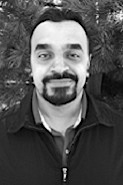
\includegraphics[width=1in,height=1.25in,clip,keepaspectratio]{bio-photos/mohammad}}]{Mohammad Bajammal}
  is currently pursuing his doctoral study at the University of British Columbia (UBC), where he obtained his masters.
  His research interests include computer vision-oriented techniques for software testing, UI development, and
  program analysis for web applications.
  He won the Distinguished Paper Award at the 2018 
  International Conference on Software Testing, Verification and Validation (ICST).
  \end{IEEEbiography}

\begin{IEEEbiography}[{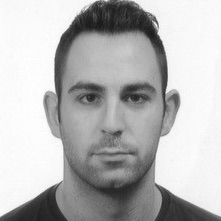
\includegraphics[width=1in,height=1.25in,clip,keepaspectratio]{bio-photos/stocco}}]{Andrea Stocco}
is a postdoctoral fellow at the Software Institute (USI), Switzerland. 
His research interests include web testing and empirical software engineering, with particular emphasis on test breakage detection and automatic repair, robustness and maintainability of test suites for web applications. He is the recipient of the Best Student Paper Award at the 16th International Conference on Web Engineering (ICWE 2016). 
He serves on the program committees of top-tier software engineering conferences such as FSE and ICST, and reviews for numerous software engineering journals including TSE, EMSE, TOSEM, JSS, and IST. 
\end{IEEEbiography}

\begin{IEEEbiography}[{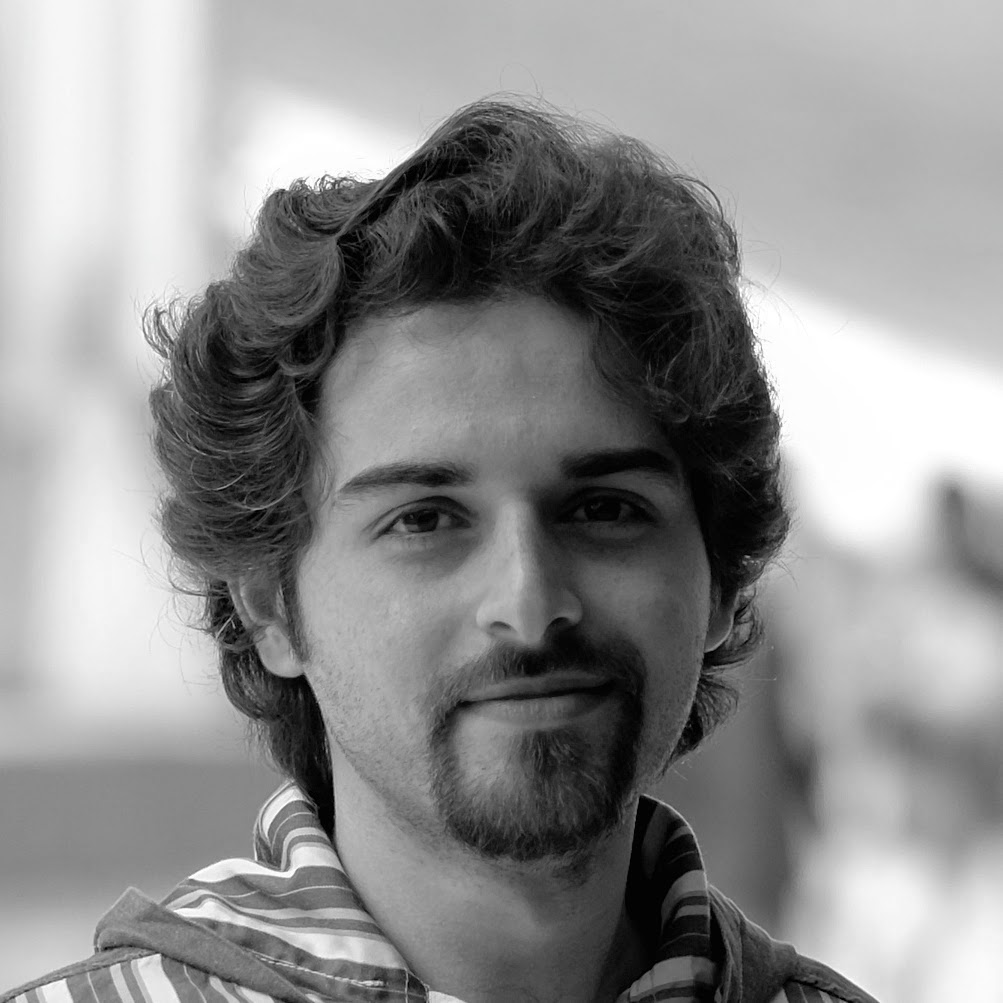
\includegraphics[width=1in,height=1.25in,clip,keepaspectratio]{bio-photos/davood.jpg}}]{Davood Mazinanian}
is postdoctoral fellow at the University of British Columbia (UBC). 
Prior to that, he was a research assistant at the 
Gina Cody School of Engineering and Computer Science, 
Concordia University, where he received his PhD in Software Engineering. 
His research interests include software maintenance and refactoring, 
program analysis, and empirical studies, with emphasis on web applications. 
He has served as a program committee member or reviewer 
for multiple software engineering conferences and journals, 
including TSE, EMSE, JSS, FSE, ICSME, and SANER.
\end{IEEEbiography}

\begin{IEEEbiography}[{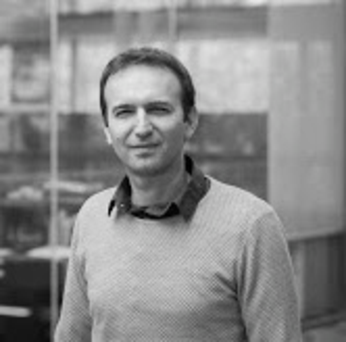
\includegraphics[width=1in,height=1.25in,clip,keepaspectratio]{bio-photos/ali}}]{Ali Mesbah}
is an associate professor at the University of British Columbia (UBC) where he leads the Software Analysis and Testing (SALT) research lab. His main area of research is in software engineering and his research interests include software analysis and testing, web and mobile-based applications, software maintenance and evolution, debugging and fault localization, and automated program repair. He has published over 60 peer-reviewed papers and received numerous best paper awards, including two ACM Distinguished Paper Awards at the International Conference on Software Engineering (ICSE 2009 and ICSE 2014). He was awarded the NSERC Discovery Accelerator Supplement (DAS) award in 2016. He is currently on the Editorial Board of the IEEE Transactions on Software Engineering (TSE) and regularly serves on the program committees of numerous software engineering conferences such as ICSE, FSE, ASE, ISSTA, and ICST.
\end{IEEEbiography}


% You can push biographies down or up by placing
% a \vfill before or after them. The appropriate
% use of \vfill depends on what kind of text is
% on the last page and whether or not the columns
% are being equalized.

%\vfill

% Can be used to pull up biographies so that the bottom of the last one
% is flush with the other column.
%\enlargethispage{-5in}



% that's all folks
\end{document}


